% Wheat Rust Prediction Report - CVPR Format
\documentclass[10pt,twocolumn,letterpaper]{article}
\usepackage[pagenumbers]{cvpr}

\usepackage{graphicx}
\usepackage{amsmath,amssymb}
\usepackage{booktabs}
\usepackage{multirow}
\usepackage{xcolor}
\usepackage{hyperref}
\usepackage[capitalize]{cleveref}
\usepackage{subcaption}

% Custom colors for tables
\definecolor{bestgreen}{HTML}{2E7D32}
\definecolor{paperblue}{HTML}{1565C0}
\definecolor{improvered}{HTML}{C62828}

\def\cvprPaperID{****}
\def\confName{CVPR}
\def\confYear{2026}

\graphicspath{{figs/}}

\begin{document}

\title{Improving Wheat Rust Disease Prediction in Ethiopia\\Using Machine Learning and Explainable AI}

\author{
Pradeep Krishnamoorthy\textsuperscript{1} \quad
Mithesh Chandrasekar\textsuperscript{1} \quad
Ruchitha Gowda\textsuperscript{1} \quad
Rohan John Varghese\textsuperscript{1}\\[4pt]
\textit{Under the guidance of:}\\
Vinutha N\textsuperscript{1}\\[6pt]
\textsuperscript{1}Department of Computer Science and Engineering\\
% \textit{Technical Report --- February 2026}
}

\maketitle

% ============================================================
\begin{abstract}
Wheat rust diseases---stem rust (\textit{Puccinia graminis} f.\ sp.\ \textit{tritici}), stripe rust (\textit{P.\ striiformis} f.\ sp.\ \textit{tritici}), and leaf rust (\textit{P.\ triticina})---are the primary biological threats to wheat production in Ethiopia, the largest wheat producer in sub-Saharan Africa. Meyer et al.\ (2021) presented the most comprehensive field surveillance analysis of wheat rusts in Ethiopia, covering ${\sim}$13,500 surveys from 2007--2019, and tested simple logistic models achieving AUC-ROC of 0.772 (stem), 0.598 (stripe), and 0.638 (leaf) under leave-one-year-out cross-validation. We extend this work by engineering domain-informed features---including growth stage, cultivar susceptibility encoding, pathogen race regime indicators, ERA5 reanalysis climate covariates, satellite-derived vegetation indices, and spatial-temporal lag features---and evaluating gradient boosting and XGBoost classifiers under the same temporal cross-validation protocol. Our best models achieve AUC of \textbf{0.833} (stem rust, +0.061), \textbf{0.719} (stripe rust, +0.121), and \textbf{0.798} (leaf rust, +0.160), representing substantial improvements across all three rust types. Spatial cross-validation confirms generalization with only 5--7\% degradation for stem and leaf rust and no degradation for stripe rust. SHAP-based interpretability analysis reveals that latitude--altitude interactions, pathogen race pressure, and crop growth stage are the dominant predictive features, providing agronomically meaningful insights for surveillance prioritization.
\end{abstract}

% ============================================================
\section{Introduction}
\label{sec:intro}

Ethiopia is the largest wheat-producing country in sub-Saharan Africa, with over 4--5 million smallholder households depending on wheat production~\cite{meyer2021}. Wheat rust diseases---caused by obligate biotrophic fungi of the genus \textit{Puccinia}---are the most devastating biotic constraint to Ethiopian wheat production. Recurrent epidemics have caused estimated losses of tens of millions of USD annually, with individual outbreaks such as the stem rust race TKTTF epidemic of 2013 causing yield losses up to 100\% on susceptible varieties~\cite{meyer2021}.

Three species of wheat rust affect Ethiopian wheat: \textbf{stem rust} (\textit{Puccinia graminis} f.\ sp.\ \textit{tritici}), which thrives at lower altitudes with warmer temperatures (optimum ${\sim}$20$^\circ$C); \textbf{stripe rust} (\textit{P.\ striiformis} f.\ sp.\ \textit{tritici}), which favors cooler, higher-altitude environments (optimum ${\sim}$12$^\circ$C); and \textbf{leaf rust} (\textit{P.\ triticina}), with intermediate temperature preferences (optimum ${\sim}$18$^\circ$C). The distinct epidemiological profiles of these three rusts---driven by different pathogen races, host variety susceptibilities, and environmental niches---necessitate separate predictive models for each.

Meyer et al.~\cite{meyer2021} presented the most comprehensive surveillance analysis of wheat rusts in Africa, using data from the RustTracker field disease surveillance system spanning 2007--2019. Their predictive modeling tested two empirical models: (1) a temporal logistic curve fitted to bi-weekly aggregated prevalence, and (2) a logistic GLM with four features (latitude, longitude, altitude, and days into season). Under leave-one-year-out cross-validation (LOYO-CV), Model 2 achieved AUC of 0.78 for stem rust but performed near-randomly for stripe rust (0.60) and leaf rust (0.66). Critically, despite recording growth stage and host cultivar for every surveyed field, neither variable was included in any predictive model.

In this work, we extend the Meyer et al.\ framework in several key directions:

\begin{enumerate}
\item \textbf{Domain-informed feature engineering}: We incorporate growth stage, time-aware cultivar susceptibility, pathogen race regime encoding, and spatial interaction terms---all derived from domain knowledge documented in the original paper but never exploited for prediction.

\item \textbf{External data integration}: We augment the survey data with ERA5 reanalysis climate variables (temperature, precipitation, humidity, vapor pressure deficit) and MODIS-derived NDVI satellite vegetation indices, addressing the primary missing biological drivers identified by Meyer et al.

\item \textbf{Non-linear ensemble models}: We evaluate gradient boosting (GB) and XGBoost (XGB) classifiers with Bayesian hyperparameter optimization, capturing feature interactions that the baseline logistic GLM structurally cannot represent.

\item \textbf{Per-rust model selection}: We identify that different model--feature combinations are optimal for each rust type, reflecting their distinct epidemiological drivers.

\item \textbf{Explainability analysis}: We employ SHAP (SHapley Additive exPlanations) to provide interpretable, agronomically meaningful insights into which features drive predictions for each rust type.

\item \textbf{Robustness validation}: We assess spatial generalization via leave-one-block-out cross-validation, model calibration via Platt scaling, and decision threshold optimization for operational deployment.
\end{enumerate}

% ============================================================
\section{Data}
\label{sec:data}

\subsection{Field Surveillance Data}

The primary dataset is the RustTracker field disease surveillance dataset from Ethiopia, covering approximately 13,500 field surveys conducted between 2007 and 2019~\cite{meyer2021}. Each survey records: geographic coordinates (latitude, longitude, altitude), survey date, wheat field area, crop growth stage, host cultivar identity, and disease incidence and severity scores for all three rust types. Following Meyer et al., we restrict analysis to 2010--2019 (yielding ${\sim}$10,300--10,400 records per rust type after quality filtering) and use the main wheat season (Meher, August--December) only.

The prediction target is binary disease presence (any non-zero incidence) for each rust type independently. Class distributions are imbalanced: stem rust is present in ${\sim}$34\% of surveys, stripe rust in ${\sim}$44\%, and leaf rust in only ${\sim}$18\%~\cite{meyer2021}.

\subsection{ERA5 Reanalysis Climate Data}
\label{sec:era5}

To incorporate the environmental drivers of rust infection, we extract monthly climate variables from the ECMWF ERA5 reanalysis dataset~\cite{era5} at each survey location. ERA5 provides global atmospheric reanalysis data at 0.25$^\circ$ spatial resolution from 1979 to the present, making it the most comprehensive and consistent source of gridded climate information available.

For each survey, we extract the following variables matched to the survey coordinates and the month of observation, as well as 1-month and 2-month lags:

\begin{itemize}
\item \textbf{2m temperature} ($t_{2m}$): Surface air temperature, used to compute thermal suitability indices based on published temperature optima for each rust species~\cite{roelfs1992}.
\item \textbf{2m dewpoint temperature} ($d_{2m}$): Used to derive relative humidity and leaf wetness proxies---critical for spore germination and infection.
\item \textbf{Total precipitation} ($tp$): Monthly and 3-month cumulative precipitation, as moisture is essential for infection processes.
\item \textbf{Surface solar radiation downwards} ($ssrd$): Proxy for cloud cover and light conditions affecting canopy microclimate.
\end{itemize}

From these raw variables, we derive biologically motivated features:

\noindent\textbf{Thermal suitability}: A Gaussian kernel centered on each rust's temperature optimum:
\begin{equation}
S_{thermal} = \exp\left(-\frac{(T - T_{opt})^2}{2\sigma^2}\right)
\label{eq:thermal}
\end{equation}
where $T_{opt}$ and $\sigma$ are species-specific parameters ($T_{opt}$ = 20, 12, 18$^\circ$C for stem, stripe, and leaf rust respectively).

\noindent\textbf{Vapor pressure deficit} (VPD): Computed from temperature and dewpoint as a proxy for atmospheric moisture stress:
\begin{equation}
\text{VPD} = e_s(T) - e_s(T_d) = 0.611 \exp\!\left(\frac{17.27T}{T+237.3}\right) - e_a
\end{equation}

\noindent\textbf{Leaf wetness index}: Combining humidity and temperature to estimate foliar wetness duration, which directly controls spore germination success.

\noindent\textbf{Infection risk index}: A composite score multiplying thermal suitability by leaf wetness, capturing the joint environmental favorability for infection.

\subsection{MODIS NDVI Satellite Data}

We extract Normalized Difference Vegetation Index (NDVI) values from the MODIS Terra satellite (MOD13A2, 1\,km resolution, 16-day composites) at each survey location. NDVI serves as a proxy for crop canopy density and vigor. Raw NDVI values proved uninformative for rust prediction (ranked 43rd out of 58 features by mutual information), consistent with the expectation that absolute greenness alone does not indicate disease status during the main growing season. We therefore engineer derived NDVI features:

\begin{itemize}
\item \textbf{NDVI anomaly}: Deviation from the climatological mean for each location--month combination, capturing below-normal greenness potentially indicative of crop stress.
\item \textbf{NDVI change}: Difference between current and 1-month lagged NDVI, where rapid decline may indicate rust damage.
\item \textbf{NDVI $\times$ altitude} and \textbf{NDVI $\times$ growth stage}: Interaction terms capturing altitude-dependent and phenology-dependent vegetation signals.
\end{itemize}

% ============================================================
\section{Methods}
\label{sec:methods}

\subsection{Feature Engineering}

Our feature engineering pipeline transforms the raw survey, climate, and satellite data into a comprehensive feature set organized into six categories:

\noindent\textbf{(1) Base geographic and temporal features}: Latitude, longitude, altitude, day of year, days into main season, bi-weekly period index, and altitude bands (discretized into 5 quantile bins).

\noindent\textbf{(2) Spatial interaction terms}: Second-order polynomial interactions including latitude$\times$altitude, longitude$\times$altitude, latitude$\times$longitude, latitude$^2$, longitude$^2$, and altitude$\times$time. These capture the non-linear spatial structure of disease risk that the baseline linear model cannot represent.

\noindent\textbf{(3) Cultivar susceptibility encoding}: Time-aware binary risk flags encoding known variety--race interactions. For example, the cultivar ``Digalu'' is encoded as high-risk for stem rust only from 2013 onward (following TKTTF incursion), and as medium-risk for stripe rust from 2016 (following PstS11 incursion). These encodings directly operationalize the boom-and-bust cycles documented by Meyer et al.

\noindent\textbf{(4) Pathogen race regime features}: Year-level indicators encoding known race incursion periods and their epidemiological impact:
\begin{itemize}
\item \textit{Stem rust}: TKTTF active/age/peak indicators, a race pressure index (0--3 scale), and a race$\times$cultivar interaction term.
\item \textit{Stripe rust}: PstS6 and PstS11 active/age/peak indicators, dual-race activity flag, and race-specific cultivar interaction terms.
\item \textit{Leaf rust}: Year-trend feature capturing the observed secular decline in leaf rust prevalence, plus endemic pressure indicators.
\end{itemize}

\noindent\textbf{(5) Climate-derived features}: ERA5-based variables as described in \cref{sec:era5}, including thermal suitability, VPD, leaf wetness, infection risk index, precipitation (current and cumulative), and temperature trend (current minus 2-month lag), each provided at current, 1-month, and 2-month lags.

\noindent\textbf{(6) Spatial-temporal lag features}: For each survey, we compute the mean disease prevalence among geographically proximate surveys from preceding months within the same LOYO fold (to prevent temporal leakage). We use four configurations: 25\,km/1-month, 50\,km/1-month, 100\,km/1-month, and 50\,km/2-month lags. Both the mean prevalence and the count of neighboring surveys are included as features, directly encoding the epidemic wave dynamics identified by Meyer et al.

Feature selection uses a two-stage filter: (1) mutual information with the target variable to remove zero-signal features, and (2) pairwise correlation filter (threshold $r > 0.85$) to remove redundant features, retaining the one with higher mutual information.

The total feature count varies by rust type due to per-rust race features, ranging from approximately 37 to 45 features after filtering.

\subsection{Models}

We evaluate three model families under the same LOYO-CV protocol as Meyer et al.:

\noindent\textbf{Logistic Regression (baseline)}: $\ell_2$-regularized logistic regression with standardized features, replicating the Meyer et al.\ Model 2. Uses only the four original features: latitude, longitude, altitude, days into season.

\noindent\textbf{Gradient Boosting Classifier (GB)}: Scikit-learn's GradientBoostingClassifier with 300 estimators, max depth 4, learning rate 0.08, and subsample 0.8. Uses the full engineered feature set.

\noindent\textbf{XGBoost Classifier (XGB)}: XGBoost with Bayesian hyperparameter optimization via Optuna~\cite{optuna} (80 trials). The objective function is the mean LOYO-CV AUC across all 10 folds, preventing per-fold overfitting. Optimized parameters include: number of estimators (342), max depth (3), learning rate (0.03), subsample (0.955), column sample rate (0.985), L1/L2 regularization ($\alpha$=4.9, $\lambda$=3.5$\times10^{-5}$), minimum child weight (17), and gamma (2.4).

We also evaluated TabNet~\cite{tabnet}, an attention-based deep learning architecture for tabular data, but found it consistently underperformed tree-based models by 6--8 AUC points, likely due to insufficient training data (${\sim}$9,000 samples per fold).

\subsection{Per-Rust Model Selection}

A key finding is that different model--feature combinations are optimal for each rust type, reflecting their distinct epidemiological drivers:

\begin{itemize}
\item \textbf{Stem rust}: XGBoost with full features (including ERA5 climate). Climate features provide +0.011 AUC, as stem rust is strongly temperature-driven.
\item \textbf{Stripe rust}: Gradient Boosting with base + race features only (no climate). Stripe rust inter-annual variability is dominated by race-driven dynamics, and climate features add noise.
\item \textbf{Leaf rust}: Gradient Boosting with base + race features only. Leaf rust is primarily spatially structured (altitude-driven), with minimal temporal climate signal.
\end{itemize}

\subsection{Evaluation Protocol}

\noindent\textbf{Leave-One-Year-Out Cross-Validation}: Following Meyer et al.\ exactly, we train on 9 years and test on the held-out year, repeating for all years 2010--2019 (10 folds). This tests the operationally relevant scenario of predicting disease in a novel year.

\noindent\textbf{Spatial Cross-Validation}: We cluster survey locations into $K=8$ spatial blocks using KMeans on (latitude, longitude) coordinates, then perform leave-one-block-out CV to assess geographic generalization independent of temporal effects.

\noindent\textbf{Calibration}: We assess probability calibration using reliability diagrams and Brier scores, and test Platt scaling (sigmoid calibration) using a temporal-aware nested CV where the most recent training year serves as the calibration set.

\noindent\textbf{Threshold Optimization}: For operational deployment, we optimize the decision threshold by maximizing F1 score across the range [0.05, 0.95] in 0.01 increments using LOYO-CV predictions.

% ============================================================
\section{Results}
\label{sec:results}

\subsection{Prediction Performance}

\cref{tab:main_results} presents the main AUC-ROC results under LOYO-CV. Our best models achieve substantial improvements over the Meyer et al.\ baseline across all three rust types. \cref{fig:auc_summary} provides a visual comparison across all models and rust types, with the paper's published AUC values shown as dashed reference lines.

\begin{table}[t]
\centering
\caption{Mean AUC-ROC under leave-one-year-out cross-validation (2010--2019). Best results per rust type in \textbf{bold}. $\Delta$ shows improvement over Meyer et al.\ baseline.}
\label{tab:main_results}
\small
\begin{tabular}{@{}llcc@{}}
\toprule
\textbf{Rust Type} & \textbf{Model} & \textbf{AUC} & \textbf{$\Delta$} \\
\midrule
\multirow{4}{*}{Stem}
  & Meyer et al.\ (LogReg)  & 0.772 & --- \\
  & GB + all features        & 0.823 & +0.051 \\
  & \textbf{XGB + all features} & \textbf{0.833} & \textbf{+0.061} \\
  & TabNet                   & 0.767 & $-$0.005 \\
\midrule
\multirow{4}{*}{Stripe}
  & Meyer et al.\ (LogReg)  & 0.598 & --- \\
  & \textbf{GB + base/race}  & \textbf{0.719} & \textbf{+0.121} \\
  & XGB + all features       & 0.700 & +0.102 \\
  & TabNet                   & 0.649 & +0.051 \\
\midrule
\multirow{4}{*}{Leaf}
  & Meyer et al.\ (LogReg)  & 0.638 & --- \\
  & \textbf{GB + base/race}  & \textbf{0.798} & \textbf{+0.160} \\
  & XGB + all features       & 0.788 & +0.150 \\
  & TabNet                   & 0.718 & +0.080 \\
\bottomrule
\end{tabular}
\end{table}

\begin{figure*}[t]
\centering
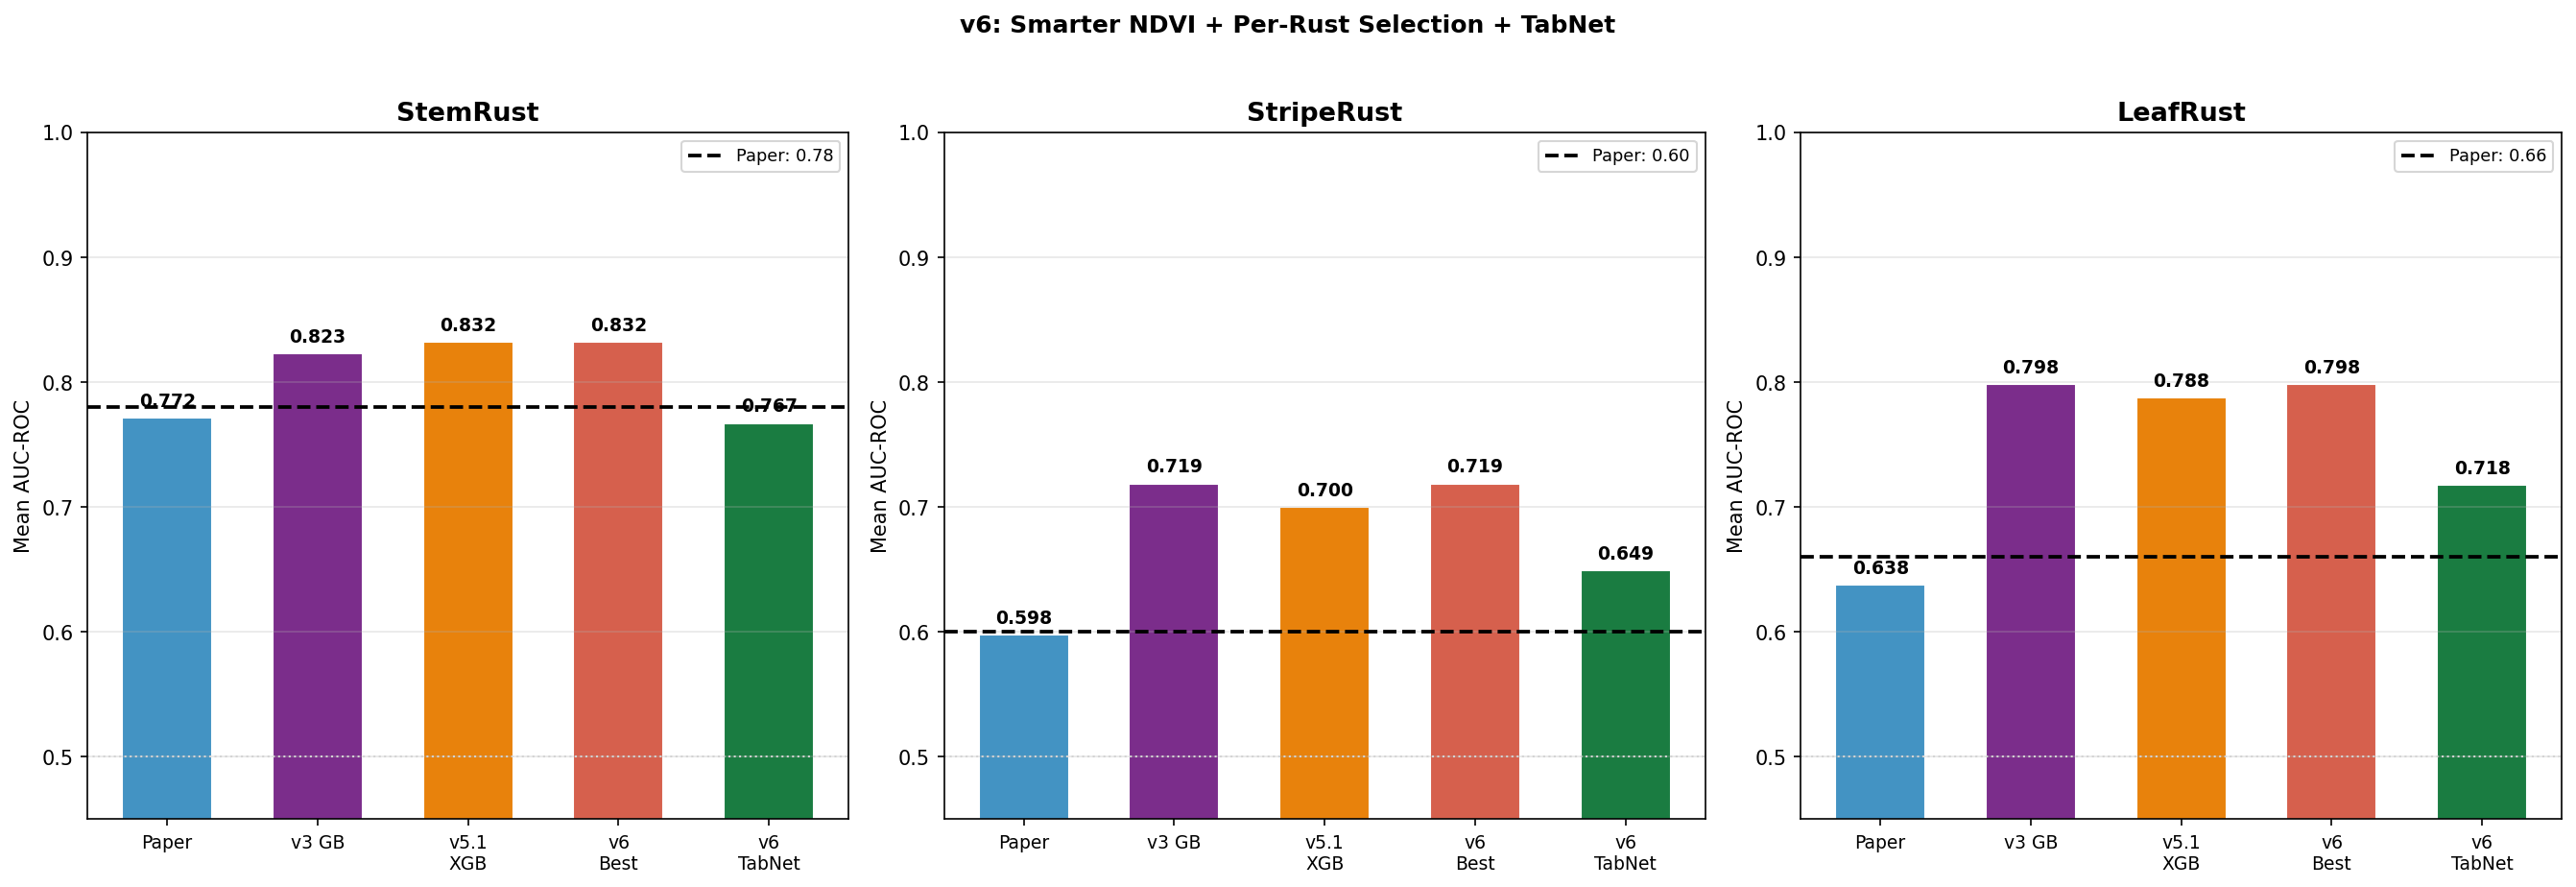
\includegraphics[width=\textwidth]{v6_summary_auc.png}
\caption{Mean AUC-ROC comparison across models and rust types. Dashed horizontal lines indicate the paper's published AUC values. Our best-of-breed models (red bars) consistently outperform all baselines. TabNet (green) underperforms tree models by 6--8 AUC points despite access to the same features.}
\label{fig:auc_summary}
\end{figure*}

The largest absolute improvement is for leaf rust (+0.160 AUC), which was previously near the threshold of meaningful predictability. Stripe rust shows a +0.121 improvement, which is notable given that the baseline was near-random. Stem rust, which already performed reasonably under the baseline, still improves by +0.061.

\cref{fig:yearly_auc} shows per-year AUC trajectories for each rust type, comparing the paper baseline, gradient boosting, XGBoost, and TabNet. The improvements are consistent across most individual years, with the largest gains in years with unusual epidemic patterns (e.g., 2012 for stripe rust: 0.388 $\rightarrow$ 0.839).

\begin{figure*}[t]
\centering
\begin{subfigure}[t]{0.33\textwidth}
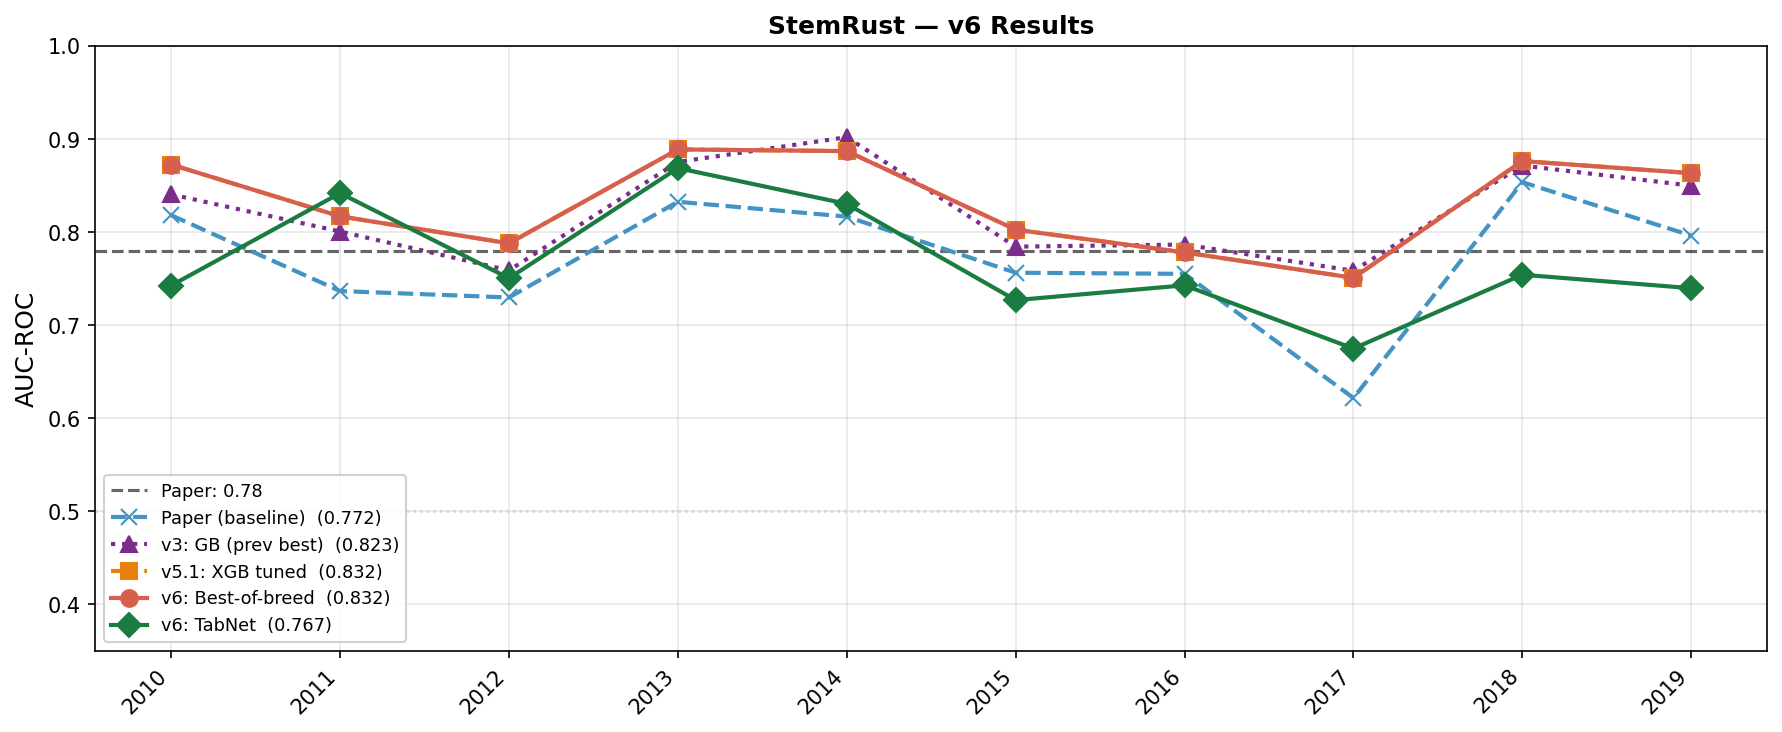
\includegraphics[width=\textwidth]{StemRust_v6_yearly_auc.png}
\caption{Stem Rust}
\end{subfigure}%
\begin{subfigure}[t]{0.33\textwidth}
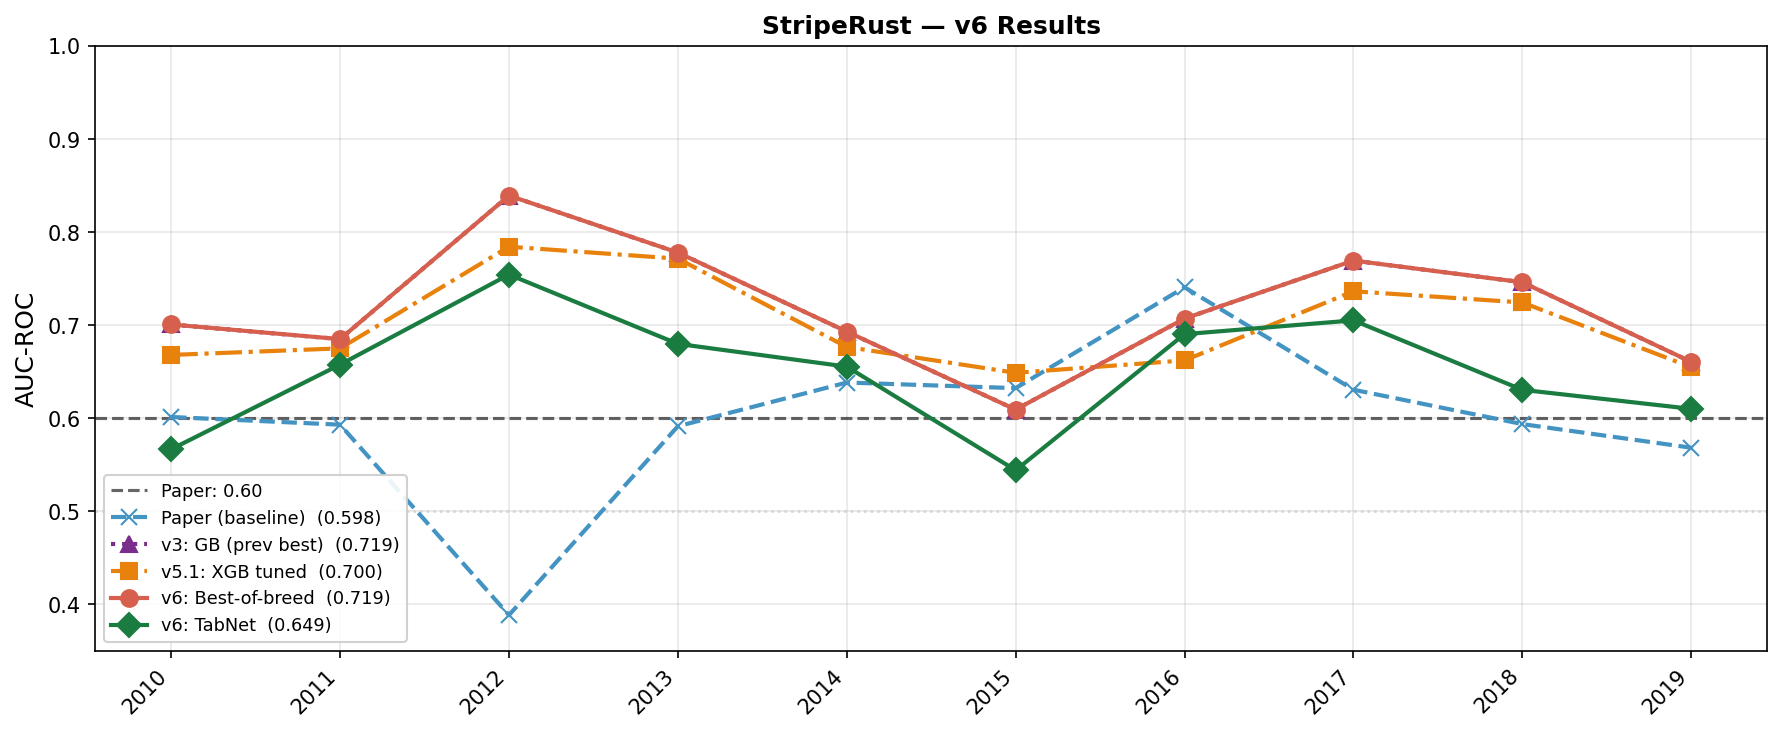
\includegraphics[width=\textwidth]{StripeRust_v6_yearly_auc.png}
\caption{Stripe Rust}
\end{subfigure}%
\begin{subfigure}[t]{0.33\textwidth}
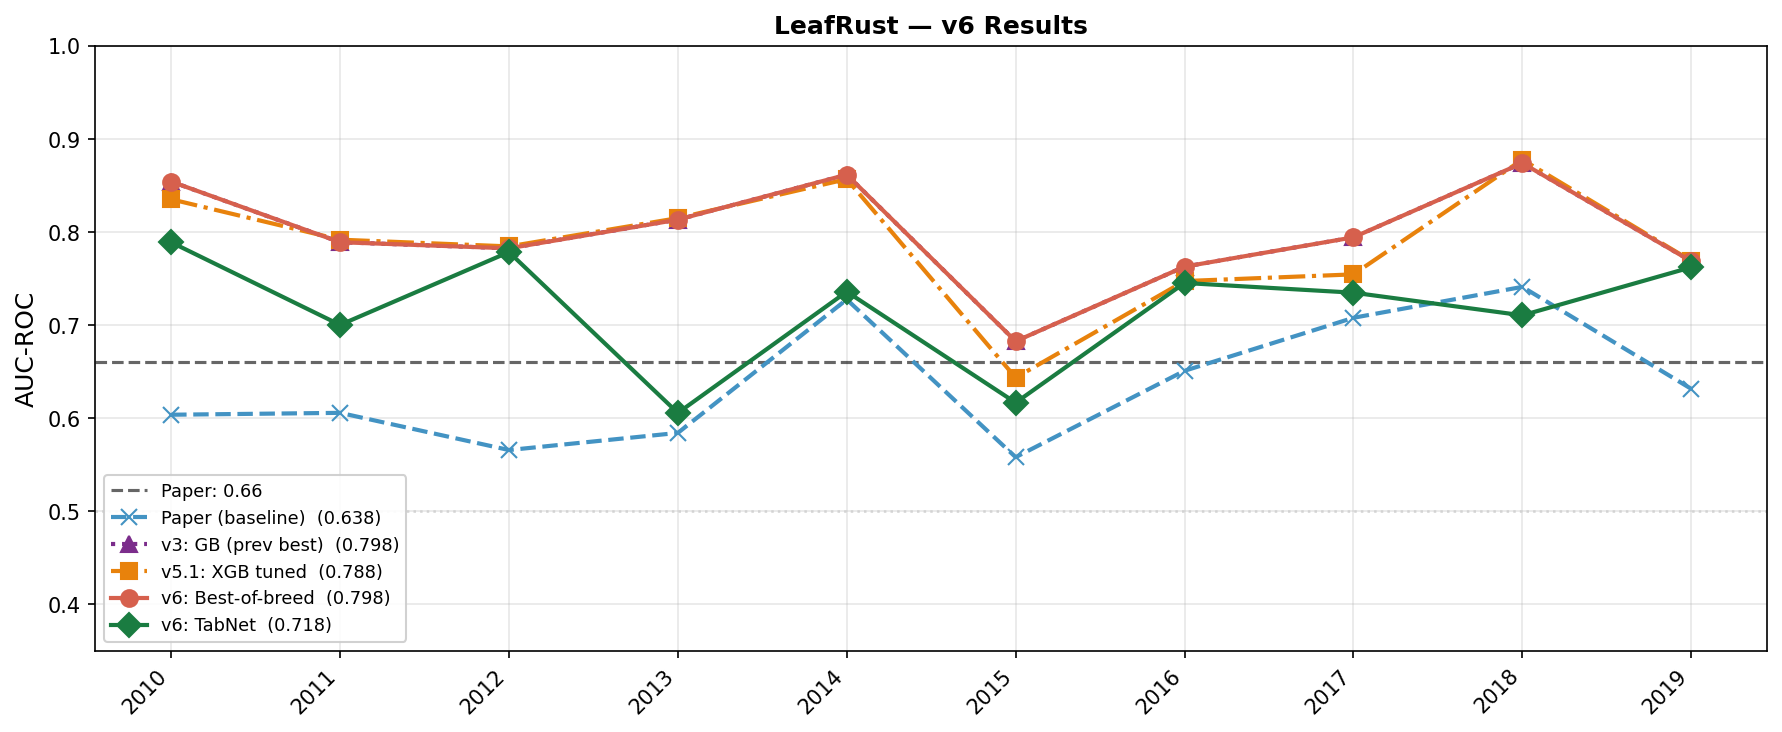
\includegraphics[width=\textwidth]{LeafRust_v6_yearly_auc.png}
\caption{Leaf Rust}
\end{subfigure}
\caption{Per-year AUC-ROC trajectories (2010--2019) for each rust type across model versions. The paper baseline (blue dashed) shows high inter-annual variability, especially for stripe and leaf rust. Our best models (red solid) achieve consistent improvements, with the largest gains in anomalous years where the baseline fails.}
\label{fig:yearly_auc}
\end{figure*}

\subsection{Spatial Generalization}

\cref{tab:spatial_cv} compares temporal (LOYO) and spatial (leave-one-block-out) cross-validation results. The spatial generalization gap is modest for stem rust (+0.056) and leaf rust (+0.069), and essentially zero for stripe rust ($-$0.006), indicating that our models generalize well to unseen geographic regions.

\begin{table}[t]
\centering
\caption{Temporal vs.\ spatial cross-validation AUC-ROC. Gap $=$ LOYO AUC $-$ Spatial AUC.}
\label{tab:spatial_cv}
\small
\begin{tabular}{@{}lccc@{}}
\toprule
\textbf{Rust Type} & \textbf{LOYO AUC} & \textbf{Spatial AUC} & \textbf{Gap} \\
\midrule
Stem rust   & 0.833 & 0.776 & +0.056 \\
Stripe rust & 0.719 & 0.725 & $-$0.006 \\
Leaf rust   & 0.798 & 0.729 & +0.069 \\
\bottomrule
\end{tabular}
\end{table}

\cref{fig:spatial_cv} provides a detailed breakdown, showing per-block spatial AUC alongside per-year temporal AUC. The spatial CV reveals that certain geographic regions (e.g., Block 1 for stem rust) are harder to predict---likely peripheral survey areas with fewer training samples---while the temporal CV shows that certain years (e.g., 2017 for stem rust) present unusual epidemic patterns that challenge all models.

\begin{figure*}[t]
\centering
\begin{subfigure}[t]{0.33\textwidth}
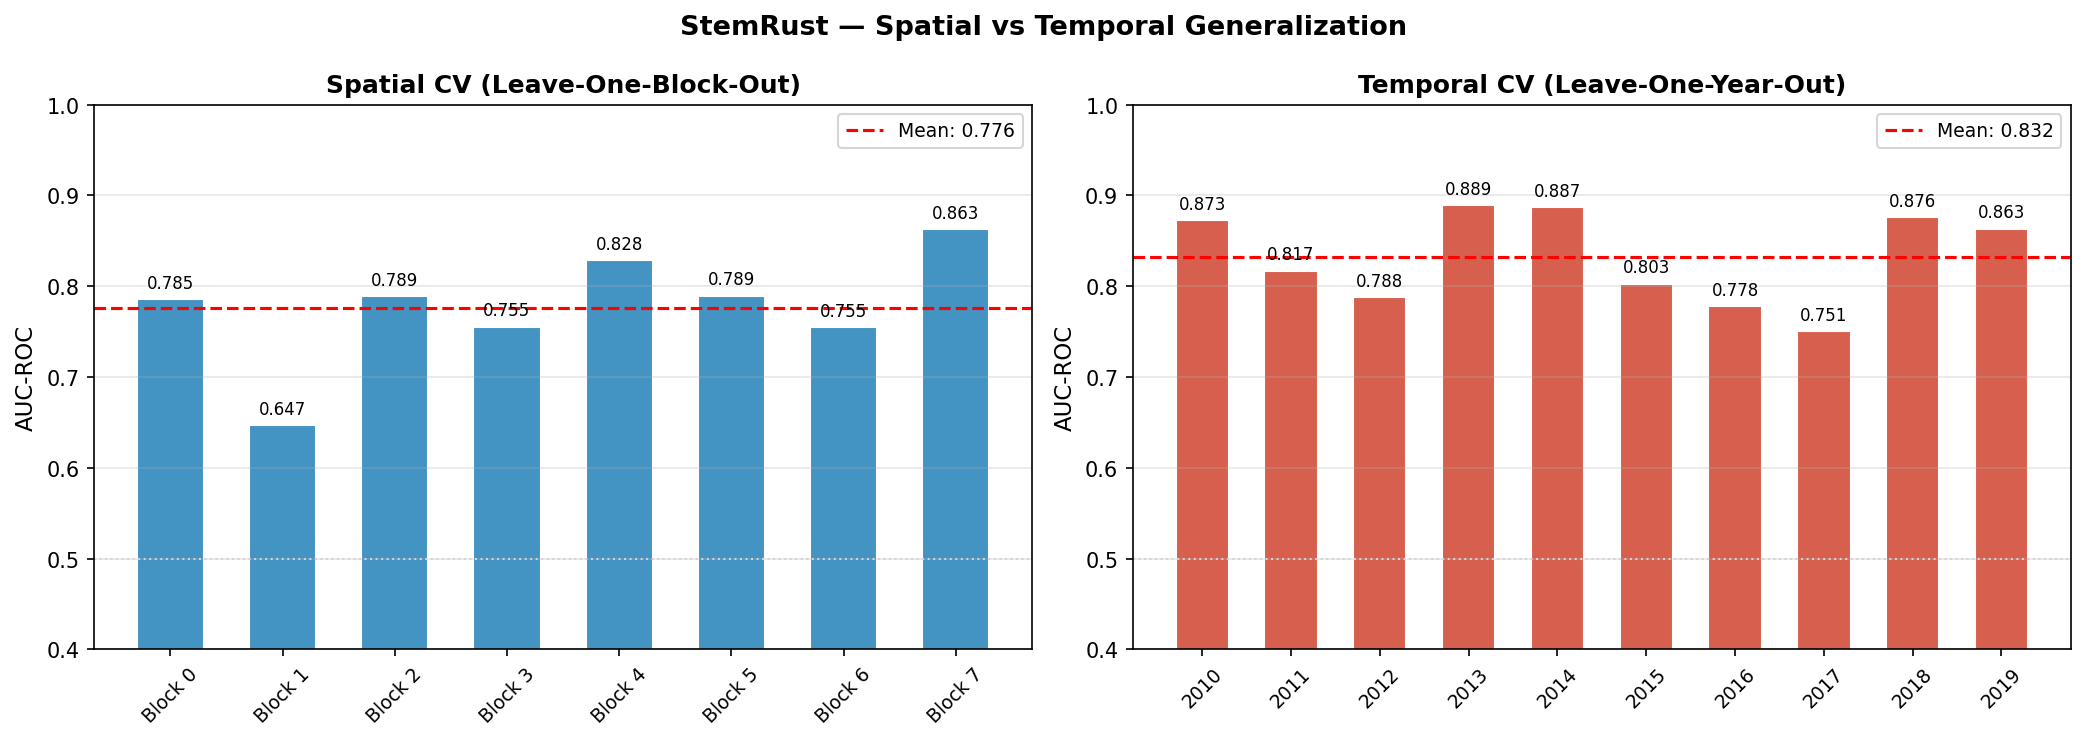
\includegraphics[width=\textwidth]{StemRust_spatial_vs_temporal.png}
\caption{Stem Rust}
\end{subfigure}%
\begin{subfigure}[t]{0.33\textwidth}
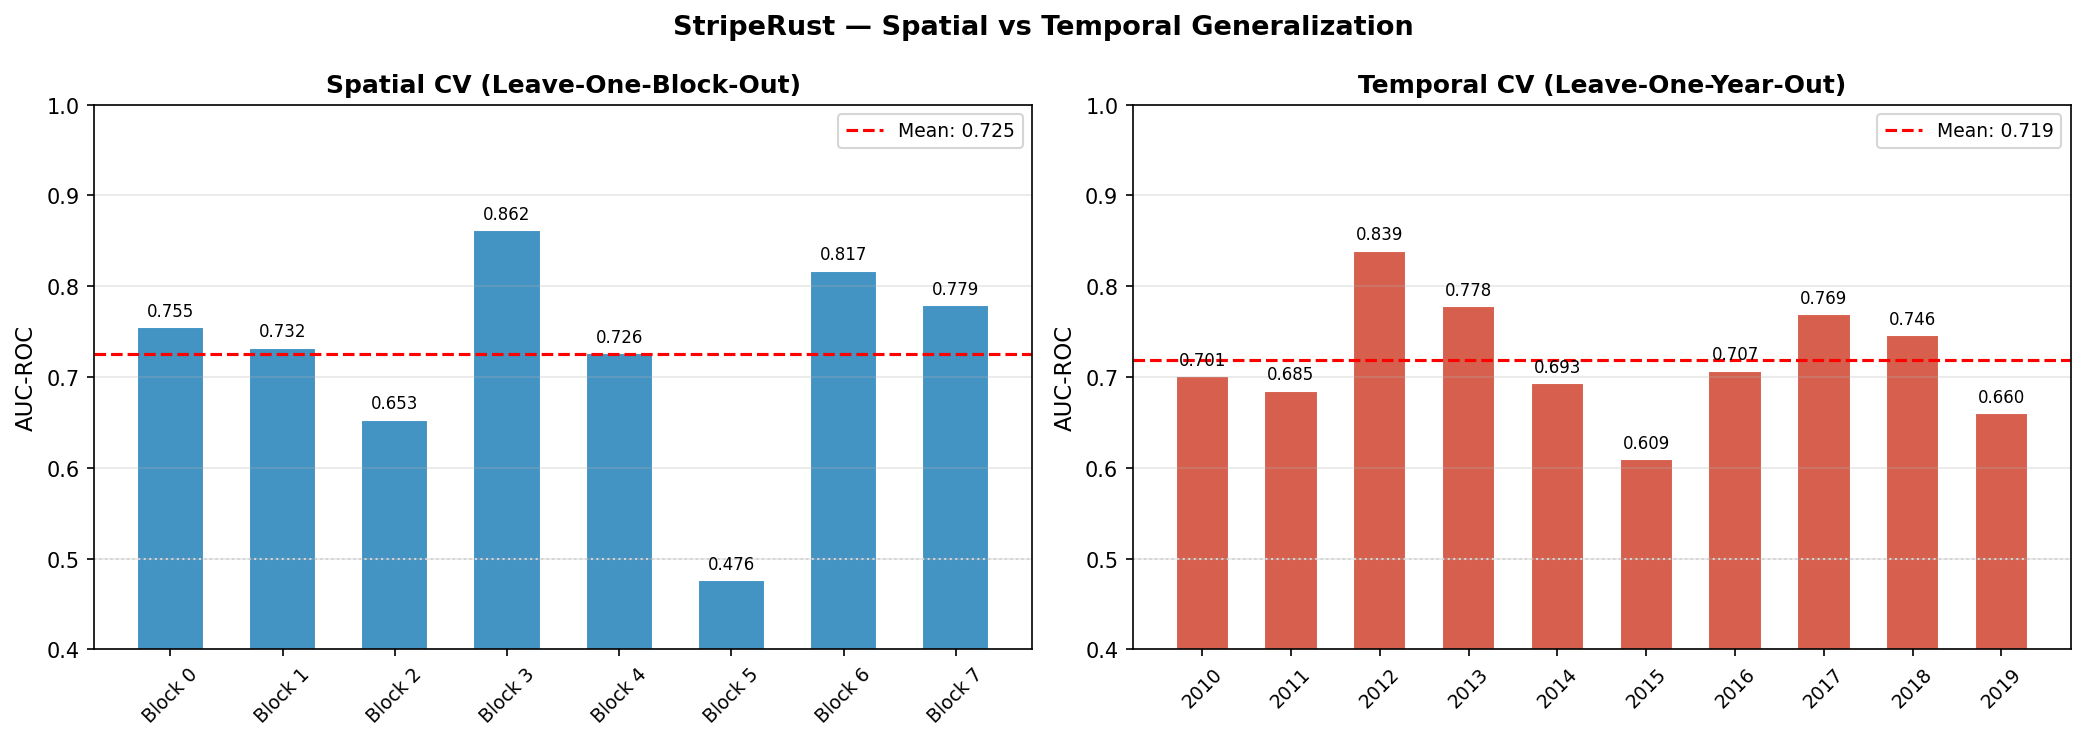
\includegraphics[width=\textwidth]{StripeRust_spatial_vs_temporal.png}
\caption{Stripe Rust}
\end{subfigure}%
\begin{subfigure}[t]{0.33\textwidth}
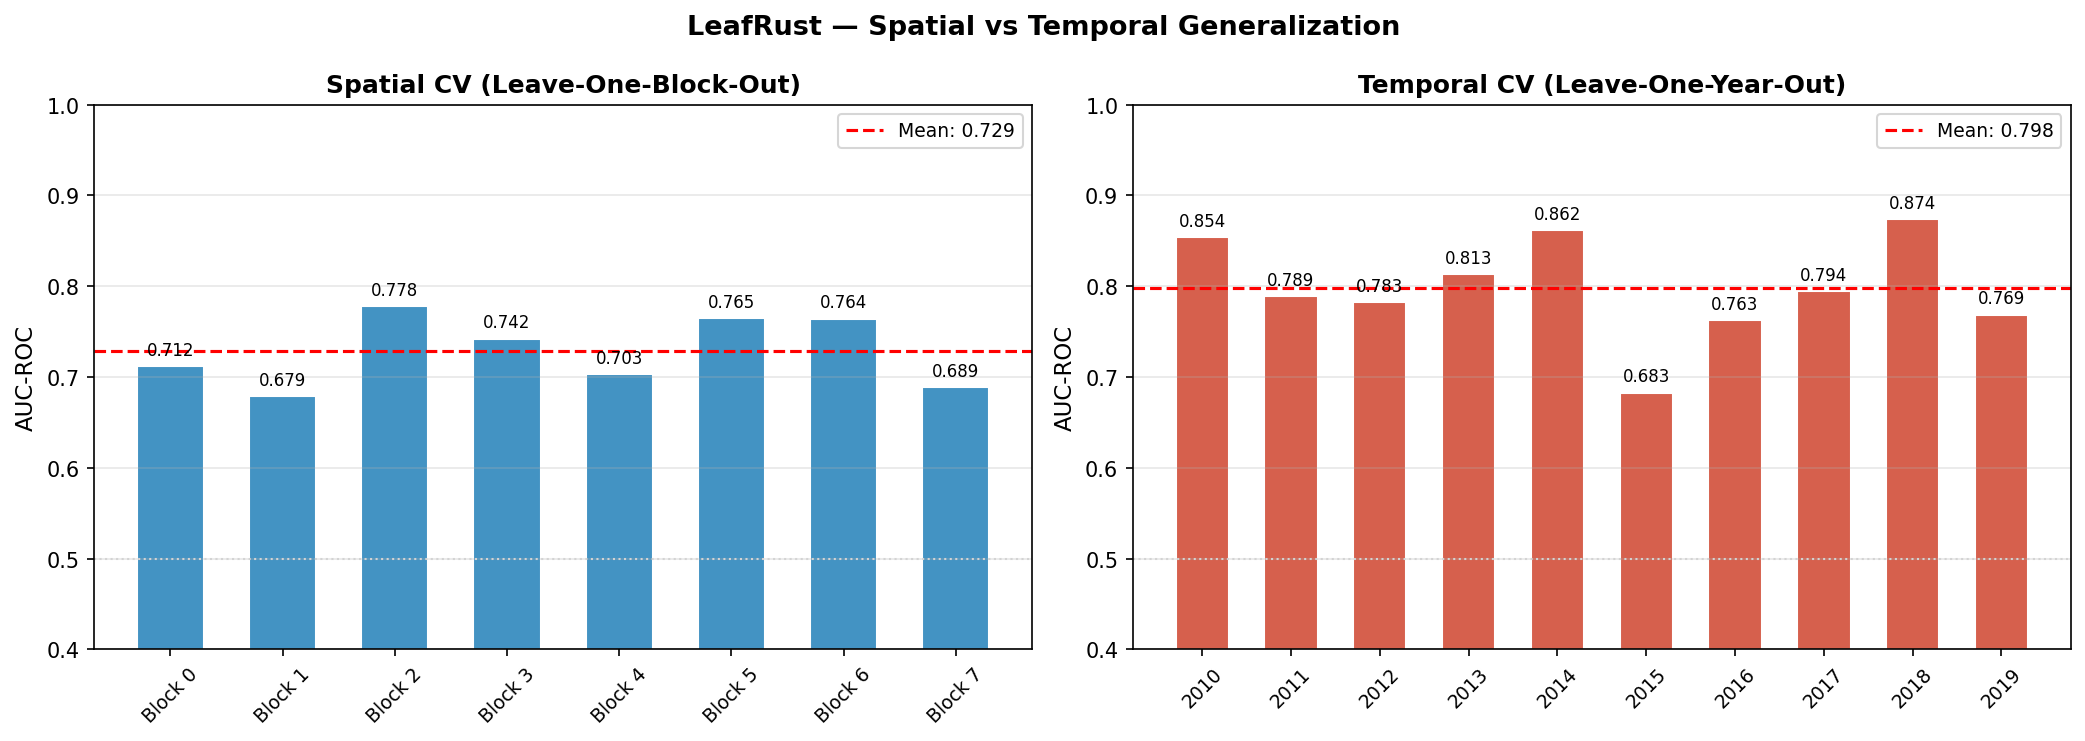
\includegraphics[width=\textwidth]{LeafRust_spatial_vs_temporal.png}
\caption{Leaf Rust}
\end{subfigure}
\caption{Spatial vs.\ temporal generalization. Left panels: per-block AUC from leave-one-block-out spatial CV ($K{=}8$). Right panels: per-year AUC from leave-one-year-out temporal CV. Red dashed lines indicate the mean AUC for each CV scheme. Stripe rust shows nearly identical means (0.725 spatial vs.\ 0.719 temporal), confirming that race-regime features generalize across both space and time.}
\label{fig:spatial_cv}
\end{figure*}

The zero gap for stripe rust is noteworthy: it confirms that the race-regime features, which encode temporal (year-level) pathogen dynamics rather than spatial patterns, are the dominant drivers for stripe rust prediction. These features generalize across locations because they represent population-level pathogen shifts affecting all regions simultaneously.

\subsection{Calibration and Threshold Optimization}

Raw model probabilities are already well-calibrated, as evidenced by Brier scores of 0.159 (stem), 0.203 (stripe), and 0.117 (leaf). Platt scaling did not improve calibration (Brier scores of 0.175, 0.206, and 0.134 respectively), indicating that the tree-based models produce reliable probability estimates without post-hoc correction. \cref{fig:calibration} shows the reliability diagrams: raw model curves (red) track the diagonal well, and Platt-scaled curves (blue) offer no improvement.

\begin{figure*}[t]
\centering
\begin{subfigure}[t]{0.33\textwidth}
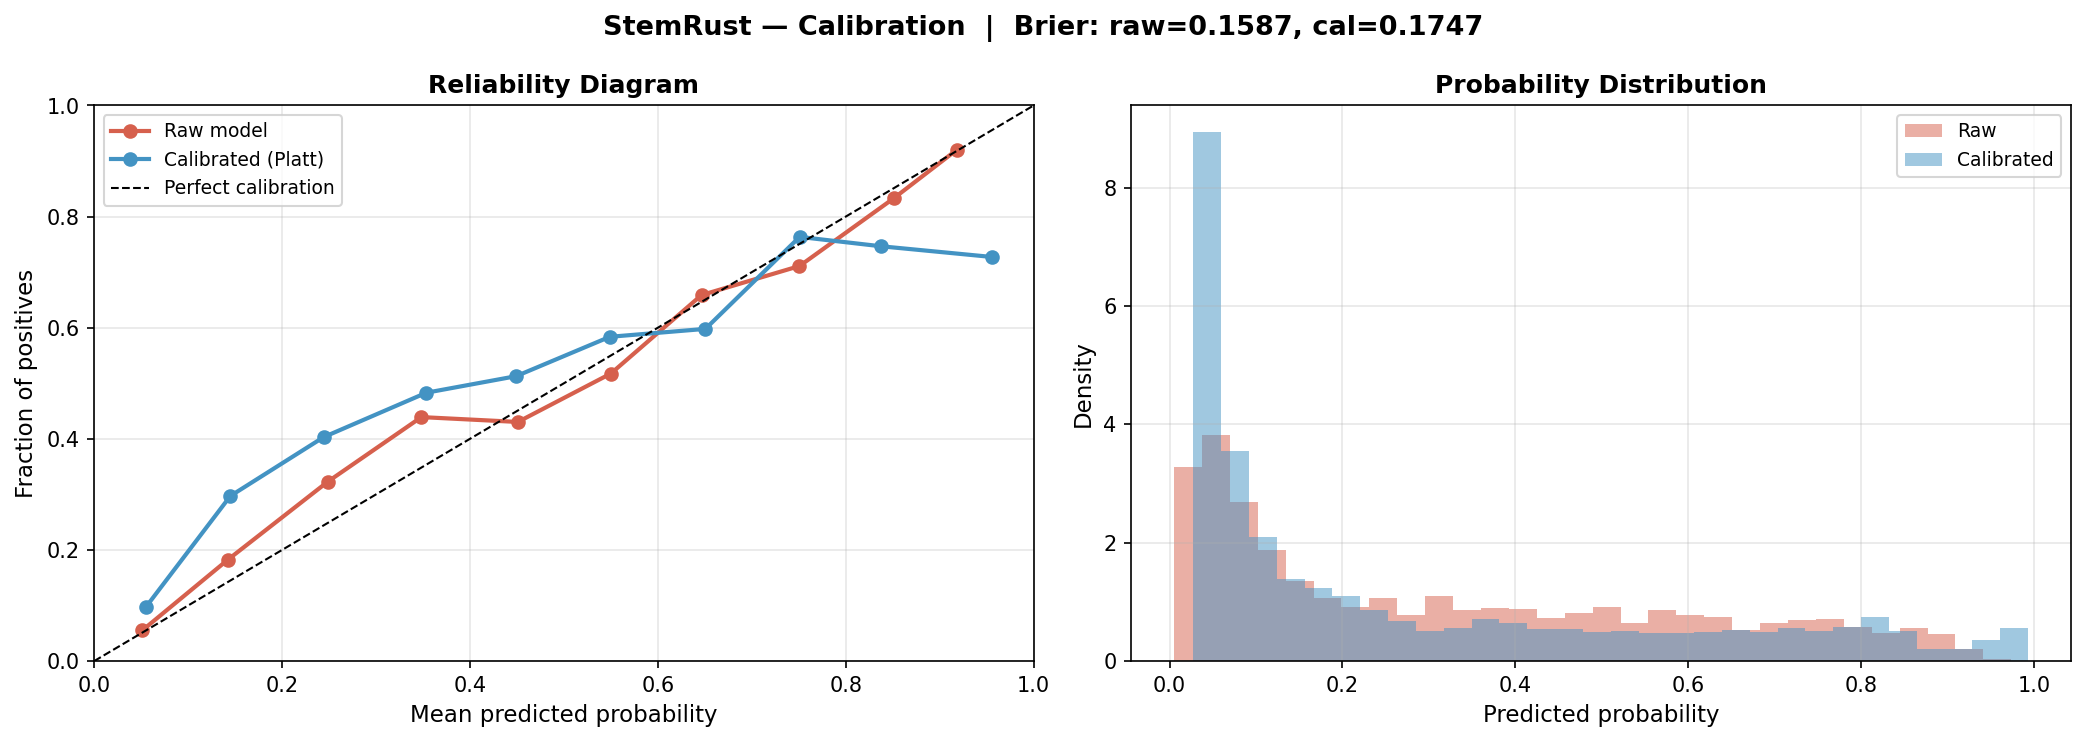
\includegraphics[width=\textwidth]{StemRust_calibration.png}
\caption{Stem Rust}
\end{subfigure}%
\begin{subfigure}[t]{0.33\textwidth}
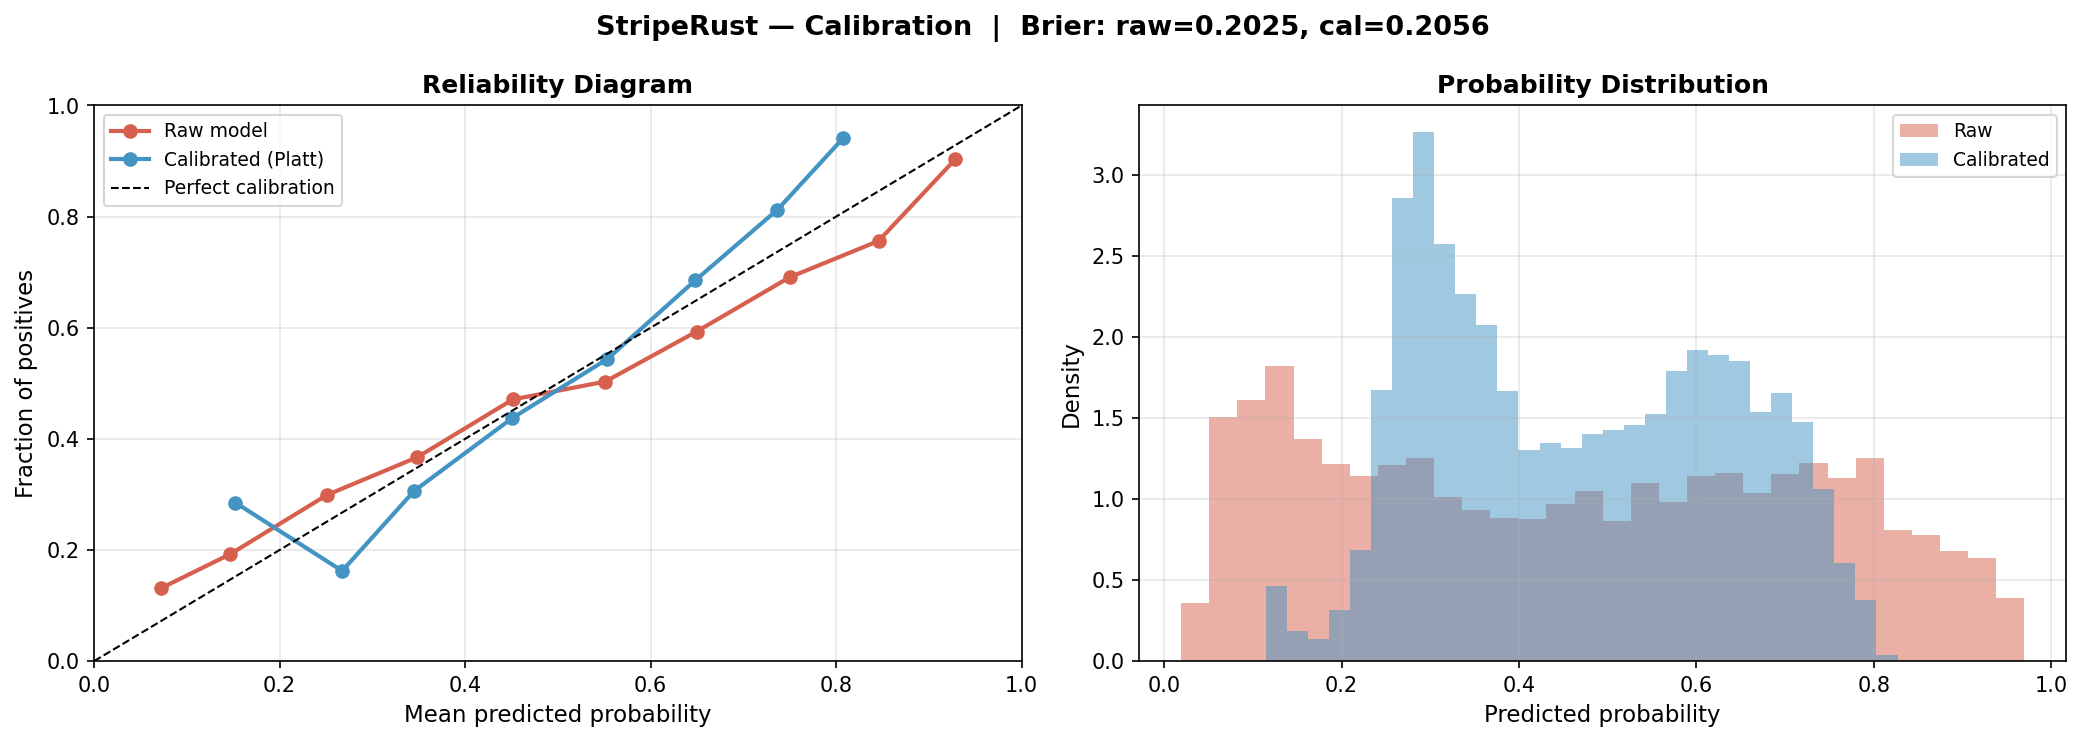
\includegraphics[width=\textwidth]{StripeRust_calibration.png}
\caption{Stripe Rust}
\end{subfigure}%
\begin{subfigure}[t]{0.33\textwidth}
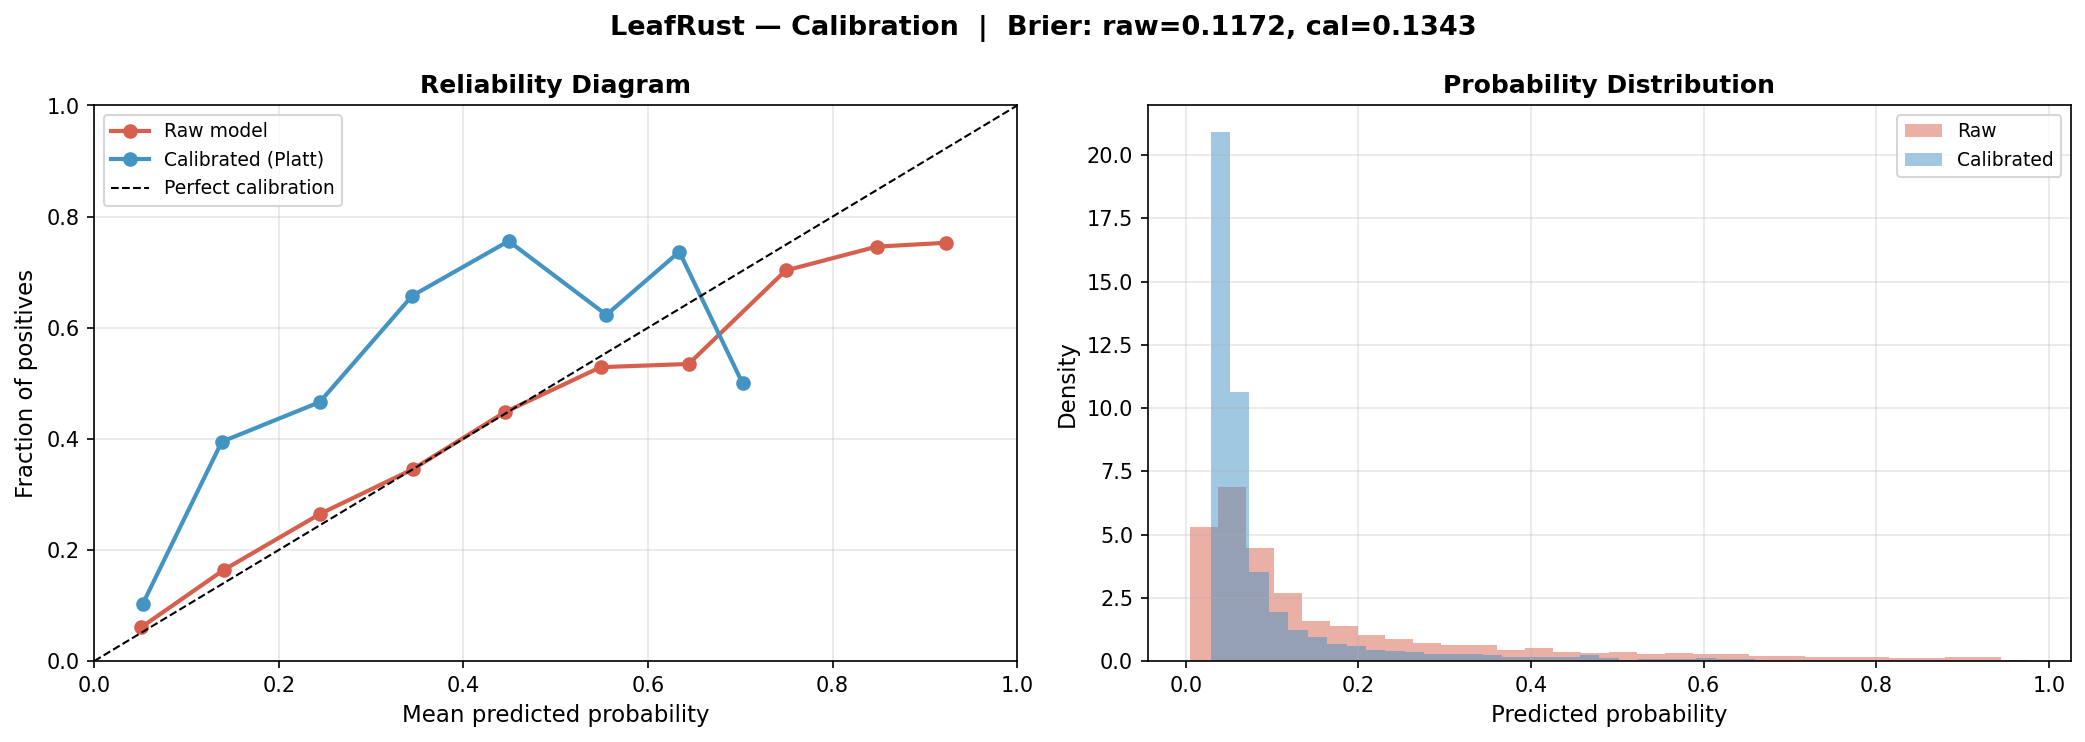
\includegraphics[width=\textwidth]{LeafRust_calibration.png}
\caption{Leaf Rust}
\end{subfigure}
\caption{Calibration analysis. Left sub-panels: reliability diagrams showing predicted probability vs.\ observed frequency. The raw model (red) closely tracks the perfect calibration diagonal (dashed black), while Platt scaling (blue) provides no improvement. Right sub-panels: predicted probability distributions for raw and calibrated models.}
\label{fig:calibration}
\end{figure*}

Threshold optimization reveals that the default 0.5 threshold is suboptimal for all three rust types due to class imbalance (\cref{tab:thresholds}). \cref{fig:threshold} visualizes F1, precision, and recall as functions of the decision threshold for each rust type, clearly showing that the F1 peak occurs well below 0.5 in all cases. The most dramatic improvement is for leaf rust, where the optimal threshold of 0.10 increases F1 from 0.094 to 0.516---reflecting the severe class imbalance (only 18\% positive) that makes the default threshold overly conservative.

\begin{table}[t]
\centering
\caption{Threshold optimization results. F1$_{0.5}$: F1 at default threshold; F1$_{opt}$: F1 at optimal threshold $t^*$.}
\label{tab:thresholds}
\small
\begin{tabular}{@{}lcccc@{}}
\toprule
\textbf{Rust} & \textbf{$t^*$} & \textbf{F1$_{0.5}$} & \textbf{F1$_{opt}$} & \textbf{$\Delta$F1} \\
\midrule
Stem   & 0.18 & 0.566 & 0.655 & +0.089 \\
Stripe & 0.35 & 0.650 & 0.680 & +0.030 \\
Leaf   & 0.10 & 0.094 & 0.516 & +0.422 \\
\bottomrule
\end{tabular}
\end{table}

\begin{figure*}[t]
\centering
\begin{subfigure}[t]{0.33\textwidth}
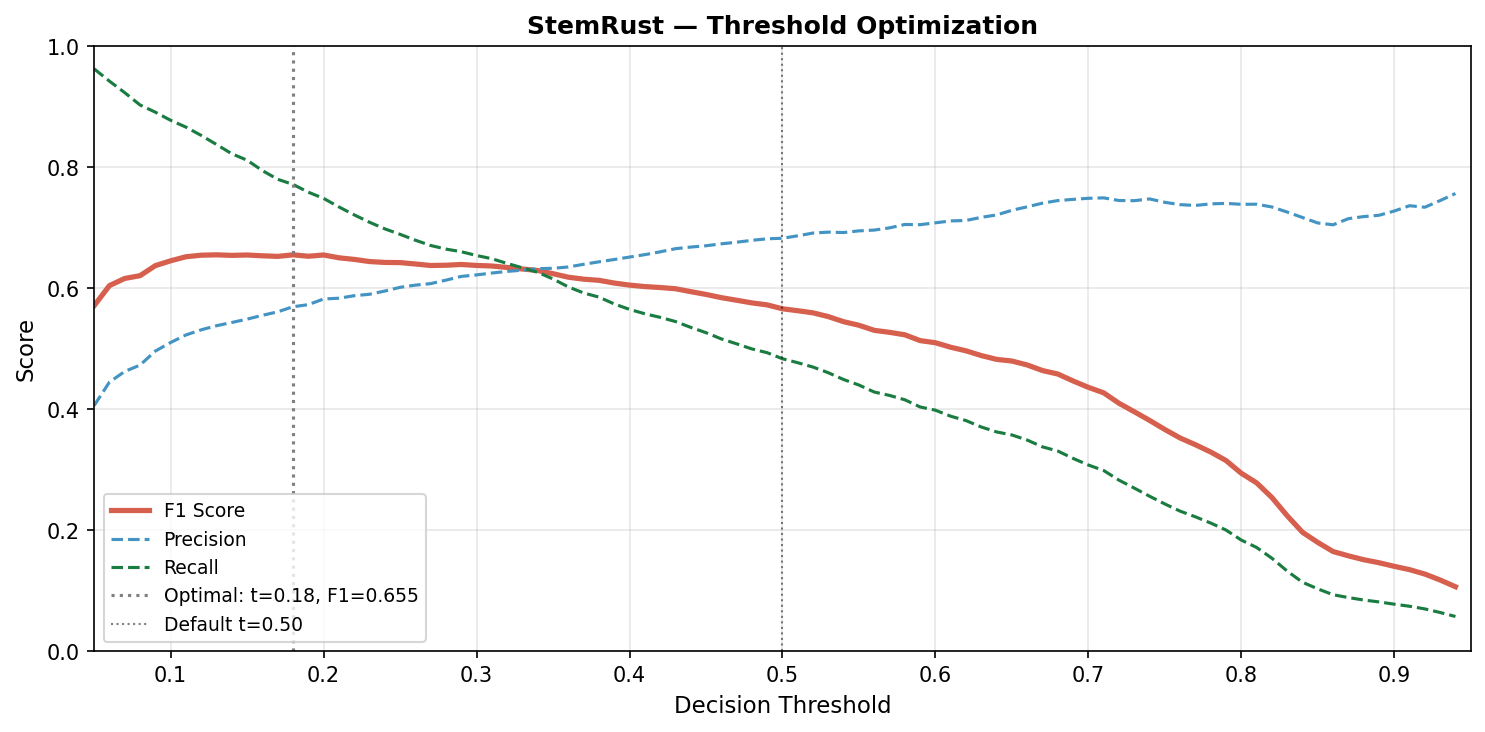
\includegraphics[width=\textwidth]{StemRust_threshold.png}
\caption{Stem Rust ($t^*{=}0.18$)}
\end{subfigure}%
\begin{subfigure}[t]{0.33\textwidth}
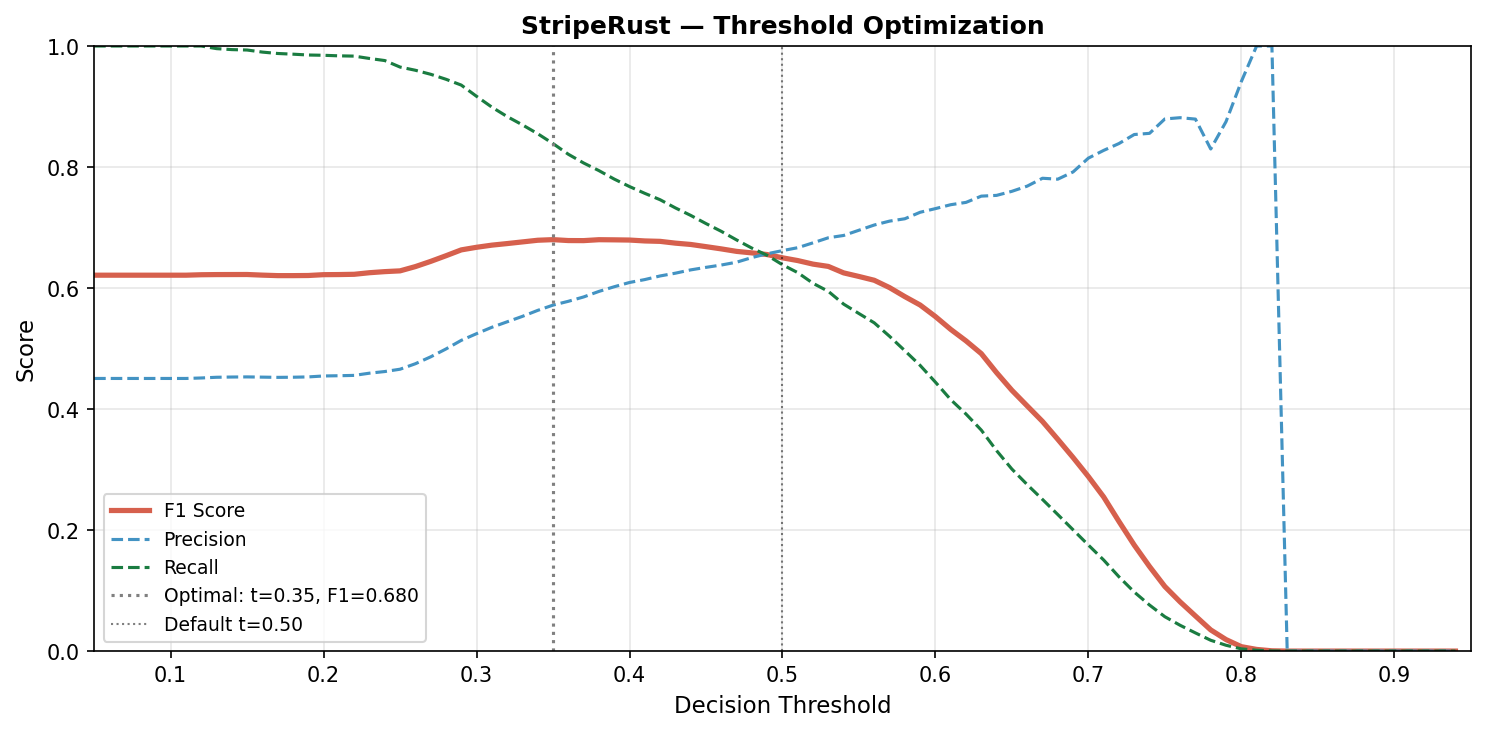
\includegraphics[width=\textwidth]{StripeRust_threshold.png}
\caption{Stripe Rust ($t^*{=}0.35$)}
\end{subfigure}%
\begin{subfigure}[t]{0.33\textwidth}
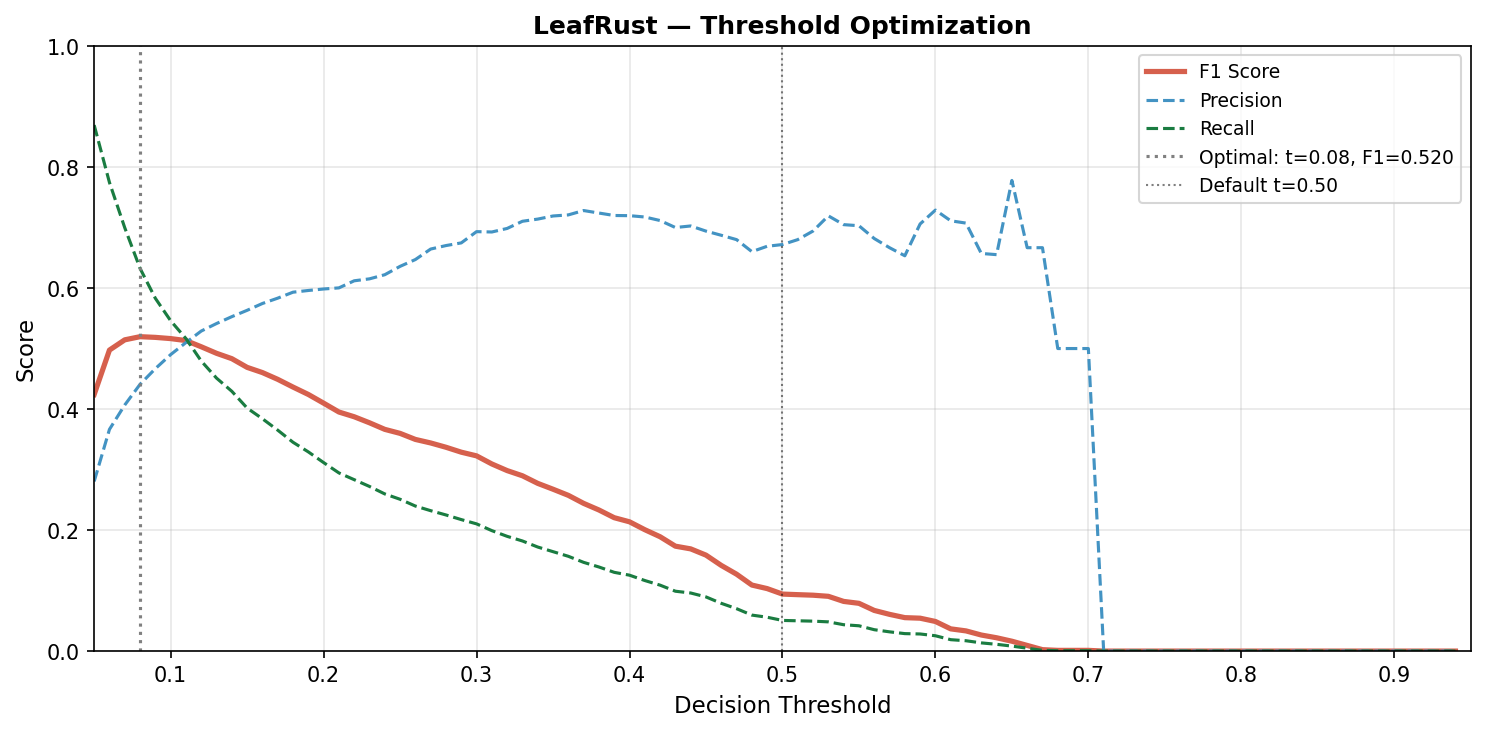
\includegraphics[width=\textwidth]{LeafRust_threshold.png}
\caption{Leaf Rust ($t^*{=}0.10$)}
\end{subfigure}
\caption{Decision threshold optimization. F1 score (red solid), precision (blue dashed), and recall (green dashed) as functions of the decision threshold. Vertical dotted lines indicate the optimal threshold (left) and the default $t{=}0.5$ (right). All optimal thresholds fall below 0.5, reflecting class imbalance. The leaf rust panel is most dramatic: the optimal threshold of 0.10 shifts from near-zero F1 to 0.516.}
\label{fig:threshold}
\end{figure*}

% ============================================================
\section{Explainability Analysis}
\label{sec:shap}

We employ SHAP TreeExplainer~\cite{lundberg2020} to compute feature importance scores for each rust type, training on the full Meher-season dataset. The results reveal distinct epidemiological signatures for each rust type.

\subsection{SHAP Feature Importance}

\cref{fig:shap_bar} shows the top-20 features ranked by mean absolute SHAP value for each rust type. The rankings reveal fundamentally different prediction drivers:

\begin{itemize}
\item \textbf{Stem rust} is dominated by \textit{geographic interactions} (Lat$\times$Alt, Lon$\times$Alt) and \textit{temporal features} (BiweekIntoSeason, GrowthStage), with race features (TKTTF age) in 4th place.
\item \textbf{Stripe rust} is dominated by a single \textit{race feature} (race\_pressure = 0.419), more than twice the next feature (Altitude = 0.189).
\item \textbf{Leaf rust} is dominated by \textit{altitude} (0.257) and the \textit{secular year trend} (0.221), reflecting its spatially structured, declining prevalence pattern.
\end{itemize}

\begin{figure*}[t]
\centering
\begin{subfigure}[t]{0.33\textwidth}
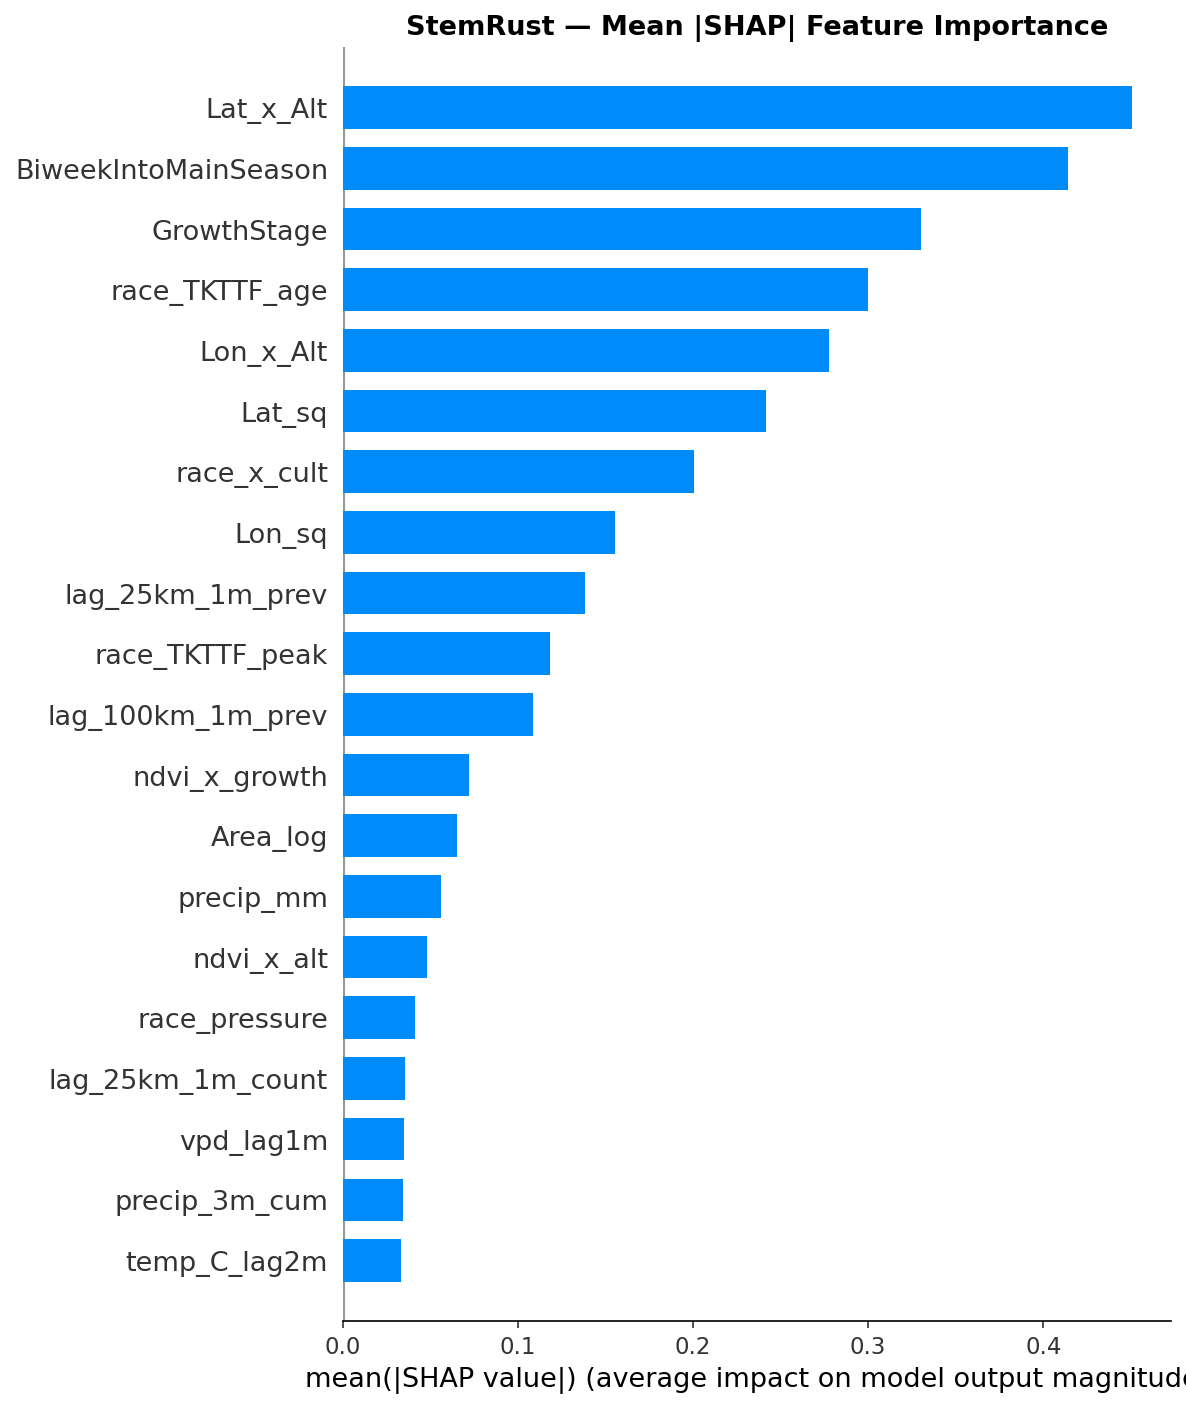
\includegraphics[width=\textwidth]{StemRust_shap_bar.png}
\caption{Stem Rust}
\end{subfigure}%
\begin{subfigure}[t]{0.33\textwidth}
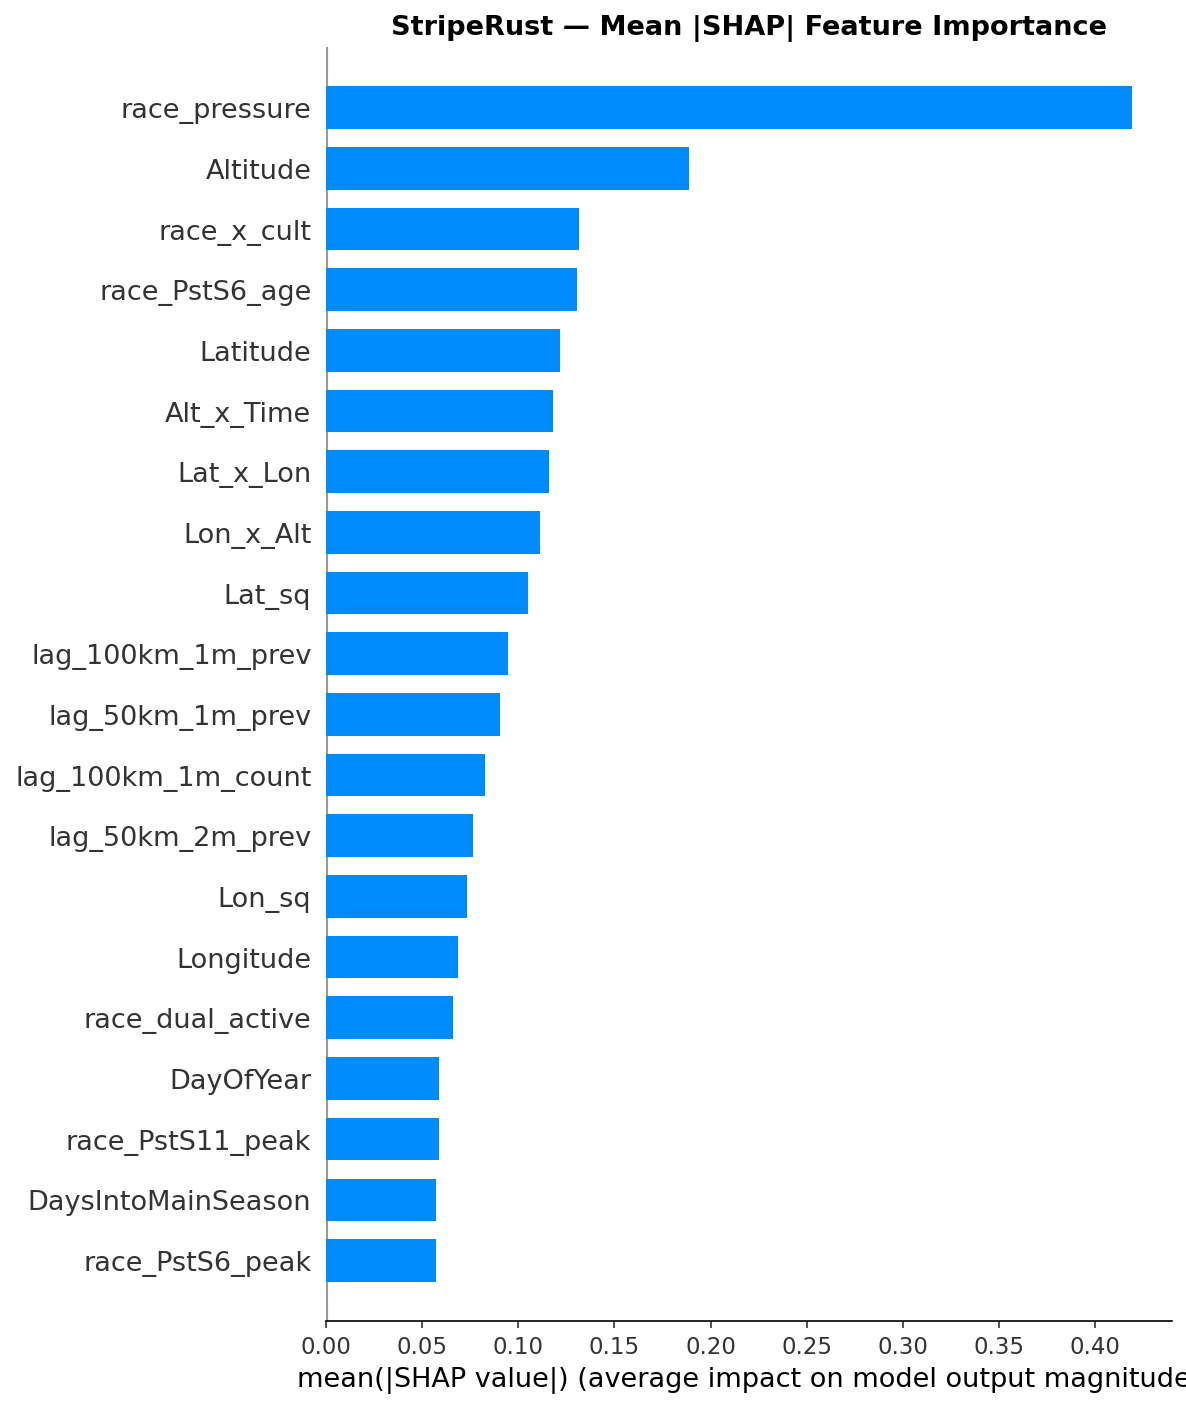
\includegraphics[width=\textwidth]{StripeRust_shap_bar.png}
\caption{Stripe Rust}
\end{subfigure}%
\begin{subfigure}[t]{0.33\textwidth}
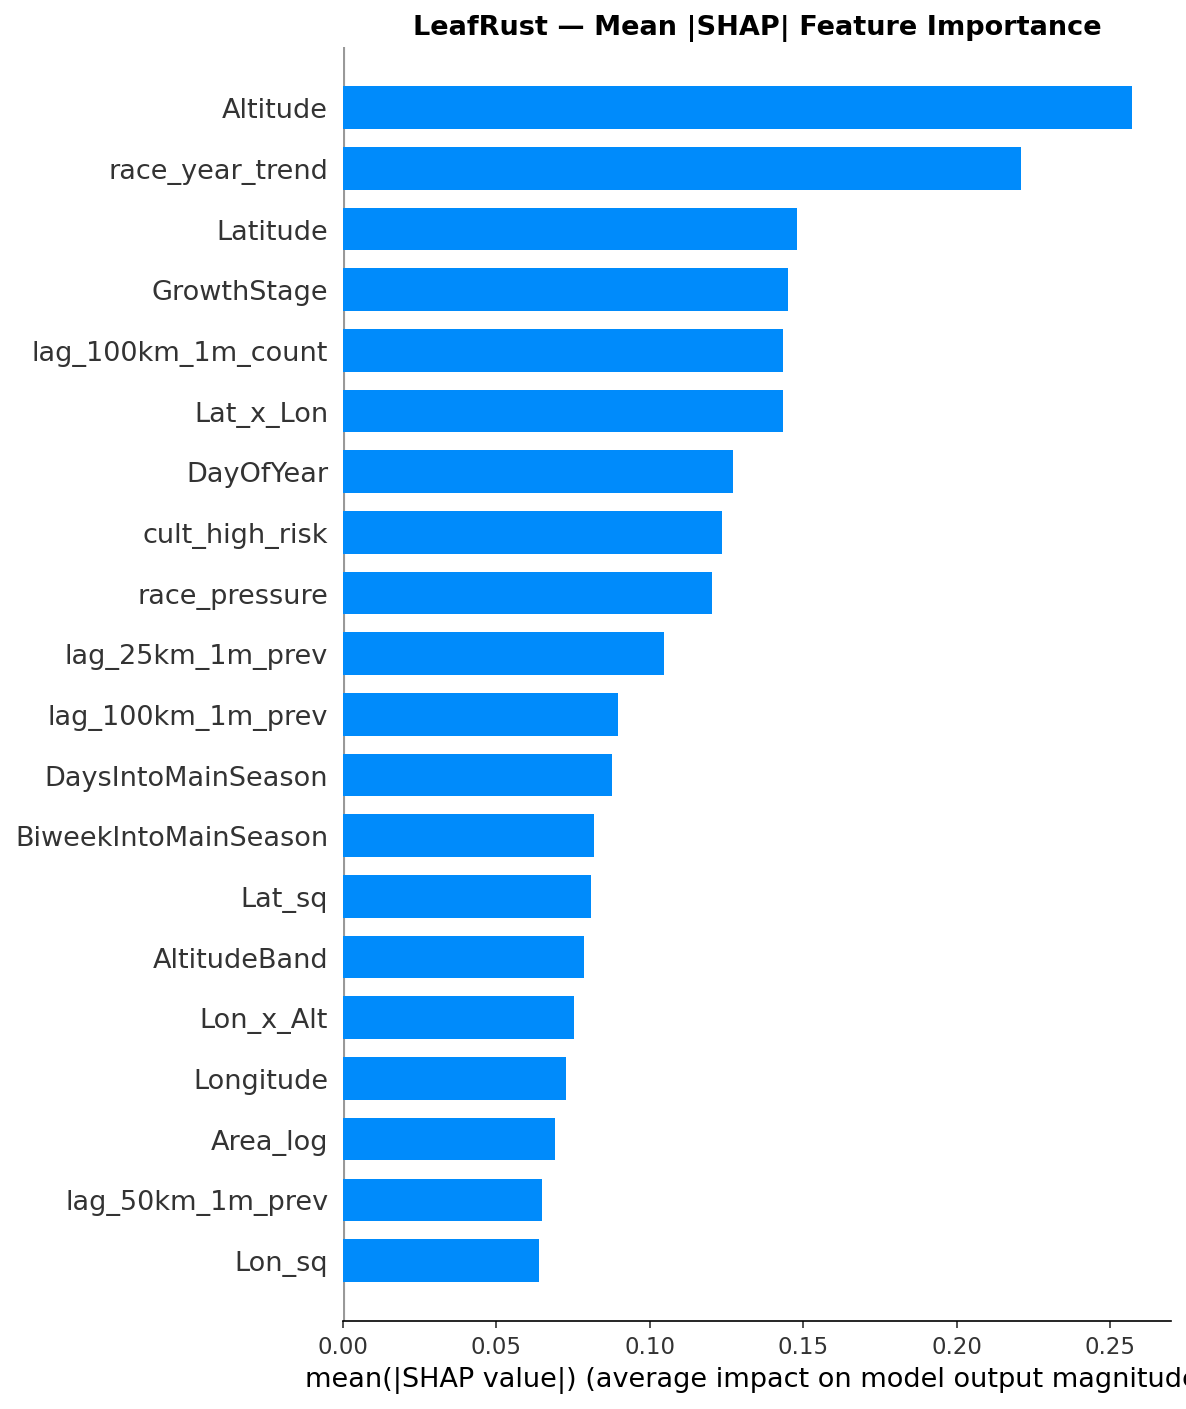
\includegraphics[width=\textwidth]{LeafRust_shap_bar.png}
\caption{Leaf Rust}
\end{subfigure}
\caption{Mean $|$SHAP$|$ feature importance for each rust type (top-20 features). Stem rust is driven by location--timing interactions; stripe rust is dominated by race\_pressure; leaf rust is driven by altitude and year trend. Climate and NDVI features (not shown in top features) rank consistently low.}
\label{fig:shap_bar}
\end{figure*}

\subsection{SHAP Beeswarm Analysis}

\cref{fig:shap_beeswarm} presents SHAP beeswarm plots revealing how individual feature values affect predictions. Each point represents a single survey, colored by feature value (red = high, blue = low), with position along the x-axis showing the SHAP contribution to the model output.

For stem rust, the Lat$\times$Alt interaction shows a clear pattern: lower values (southern, lower-altitude locations) push predictions toward disease presence (positive SHAP), consistent with the documented south-north gradient in stem rust prevalence. For stripe rust, race\_pressure shows a clean separation between low-pressure years (negative SHAP, pushing toward absence) and high-pressure years (positive SHAP). For leaf rust, high altitude values suppress disease prediction (negative SHAP for high values), consistent with the known decline of leaf rust prevalence at higher elevations.

\begin{figure*}[t]
\centering
\begin{subfigure}[t]{0.33\textwidth}
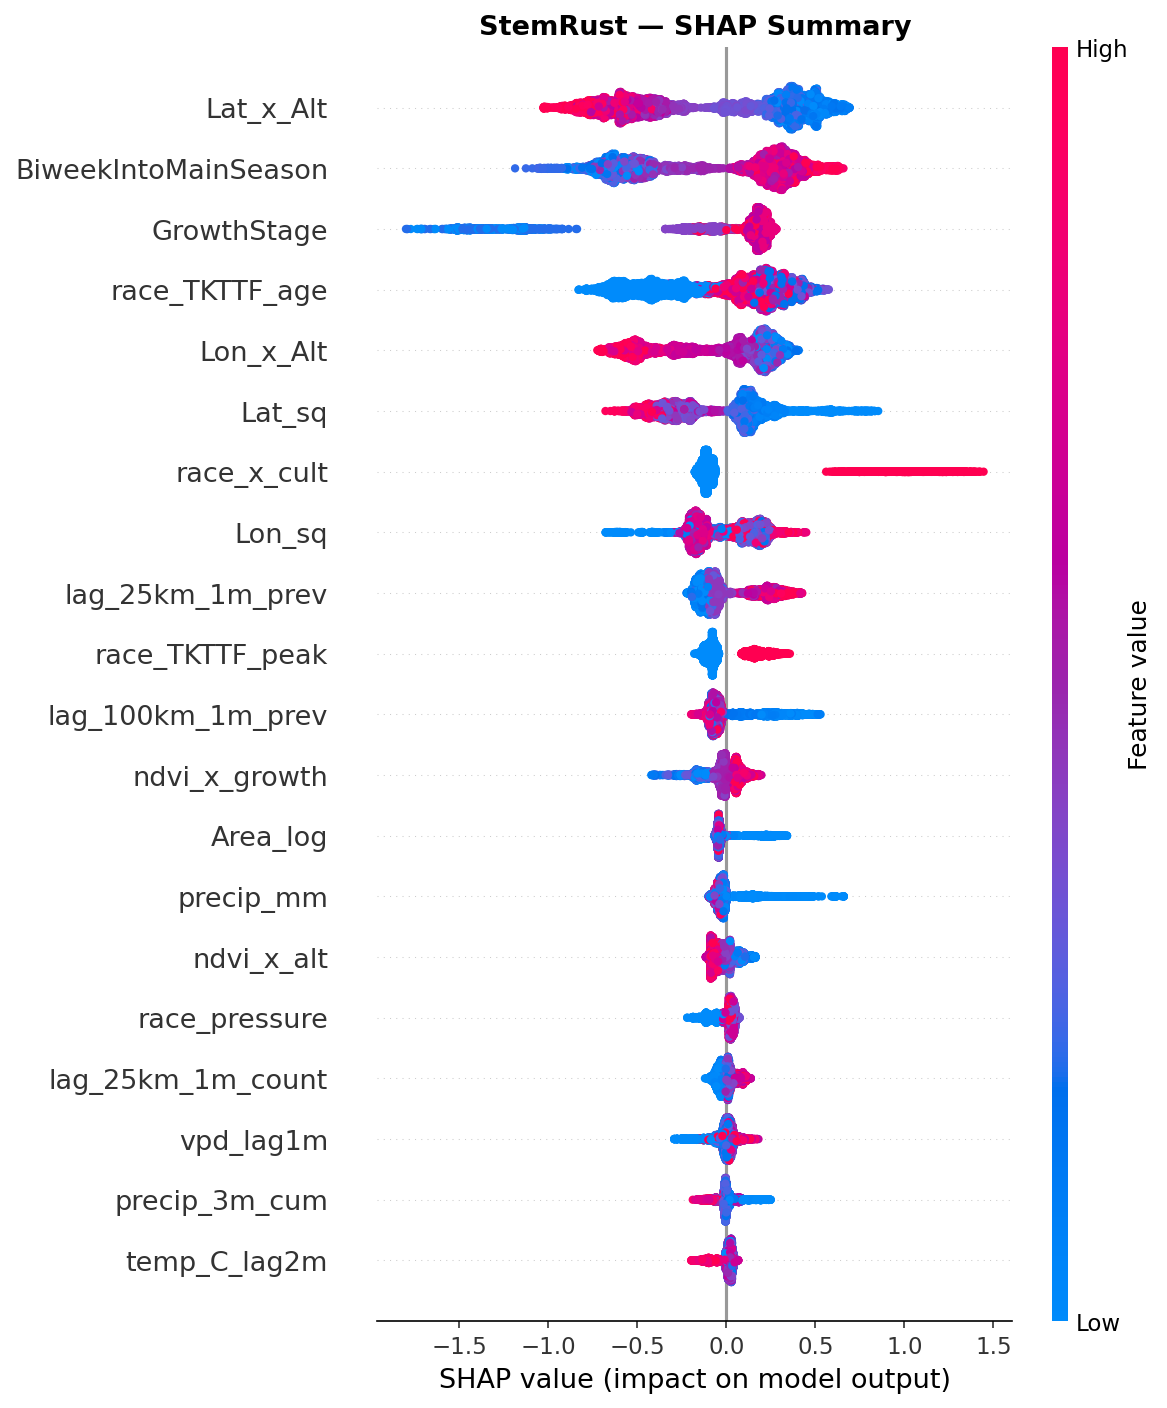
\includegraphics[width=\textwidth]{StemRust_shap_summary.png}
\caption{Stem Rust}
\end{subfigure}%
\begin{subfigure}[t]{0.33\textwidth}
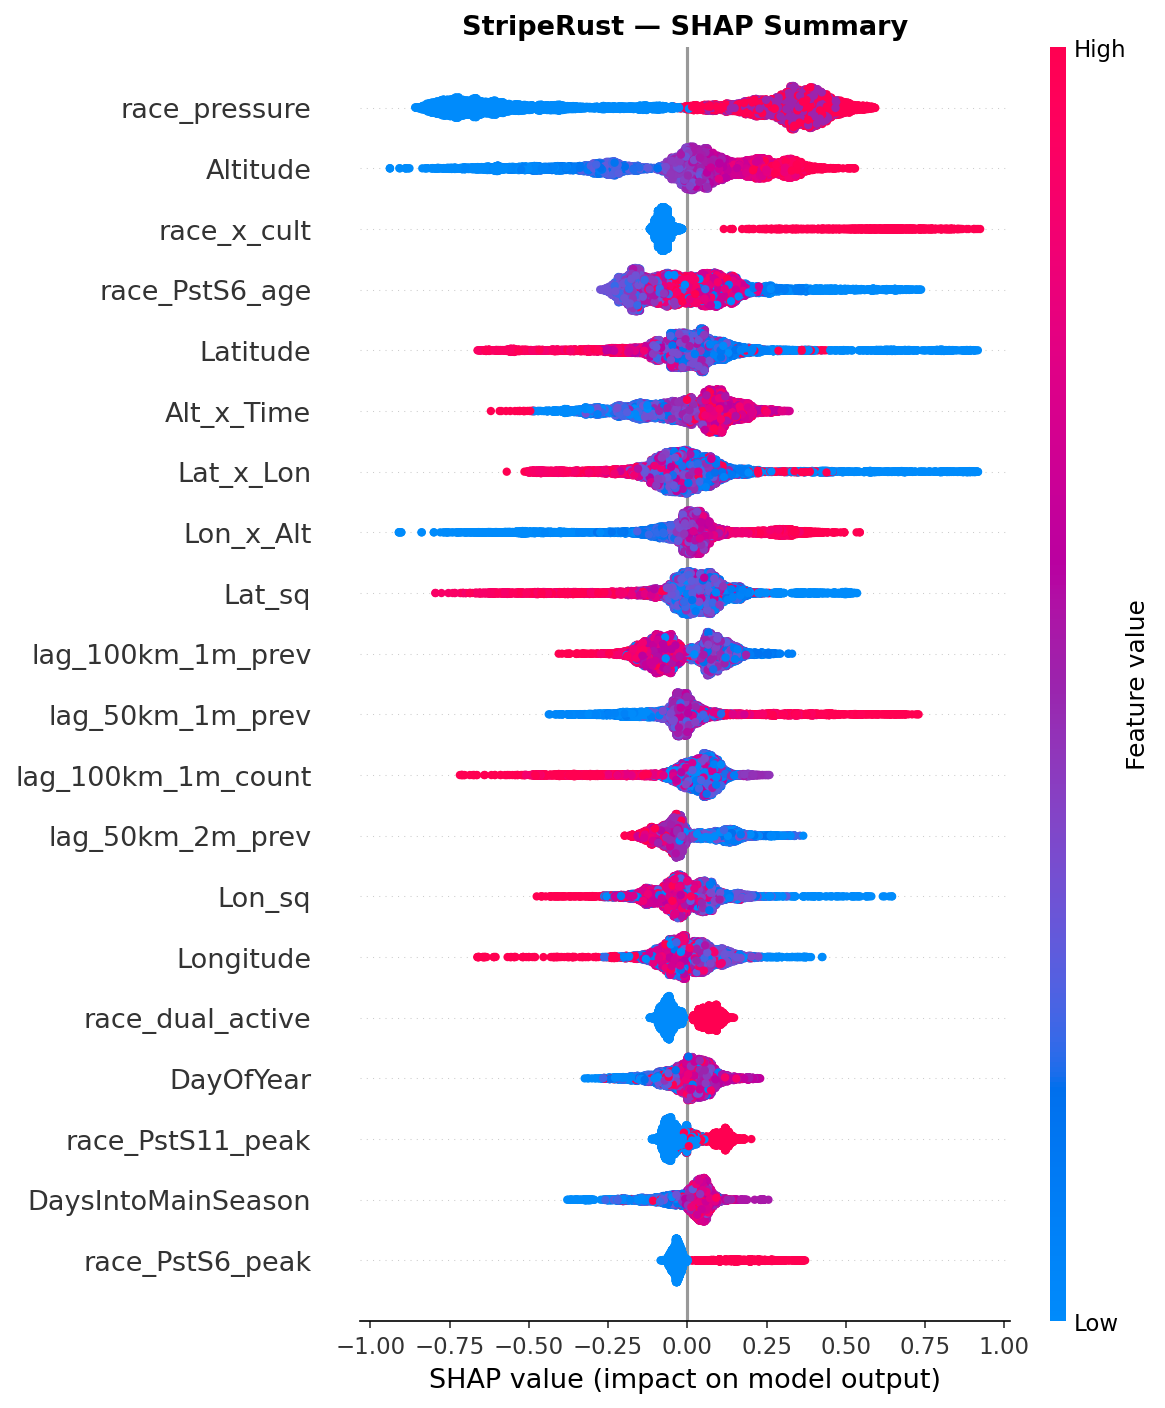
\includegraphics[width=\textwidth]{StripeRust_shap_summary.png}
\caption{Stripe Rust}
\end{subfigure}%
\begin{subfigure}[t]{0.33\textwidth}
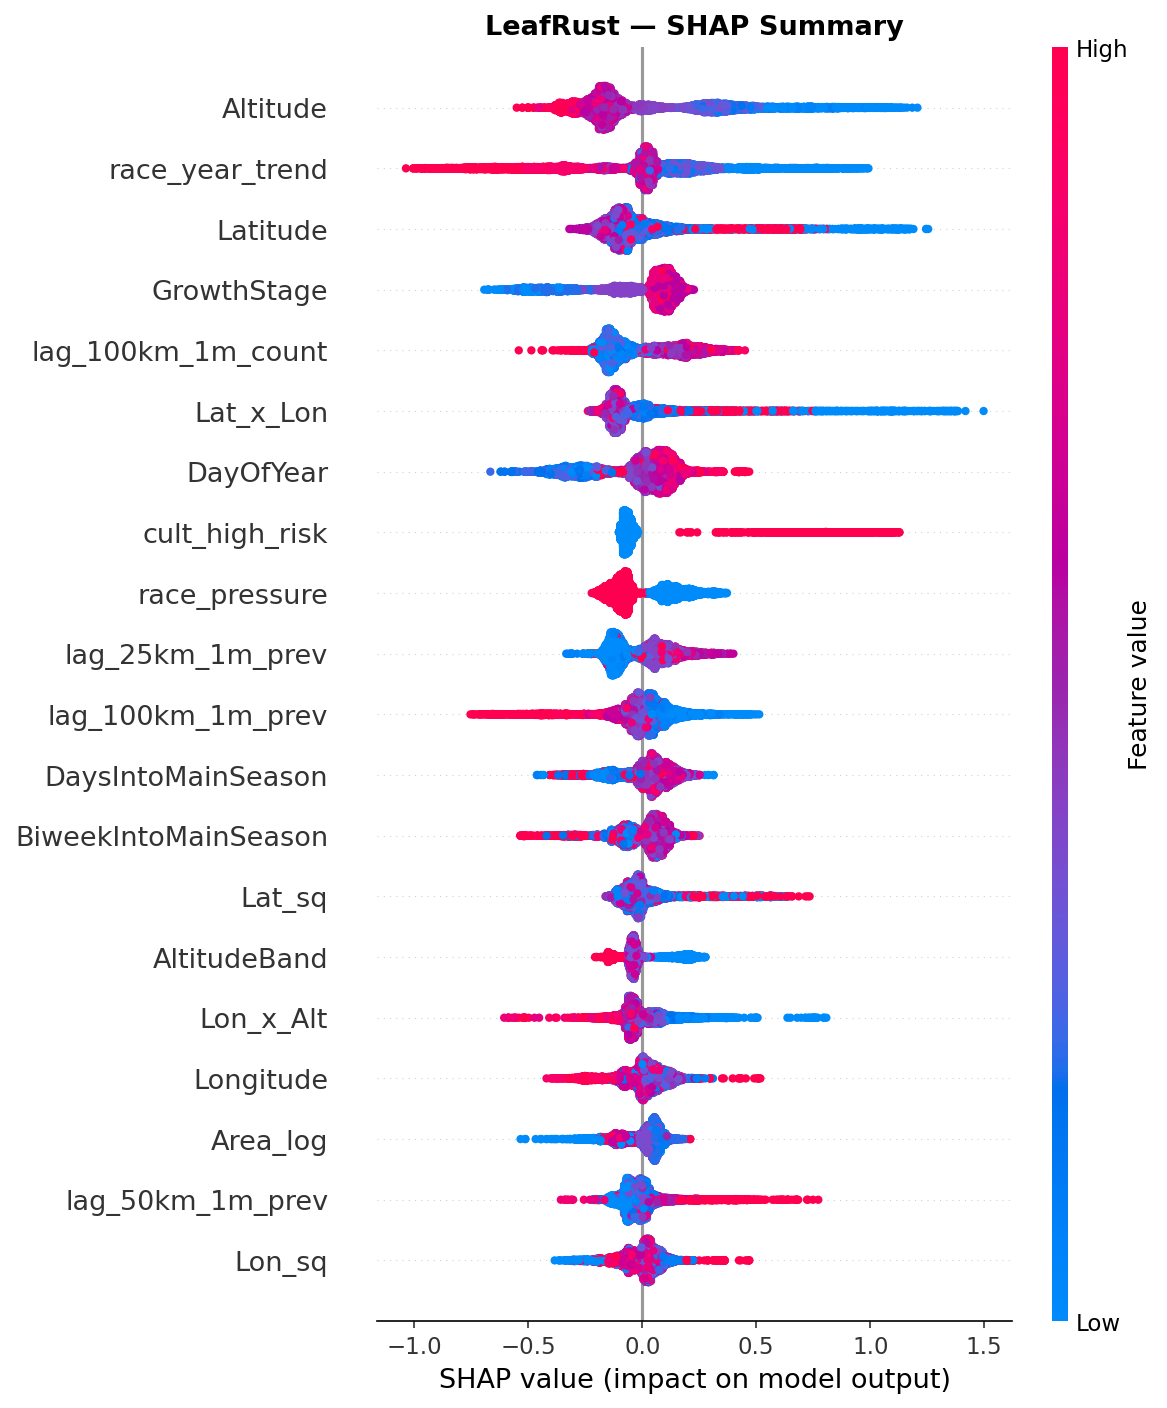
\includegraphics[width=\textwidth]{LeafRust_shap_summary.png}
\caption{Leaf Rust}
\end{subfigure}
\caption{SHAP beeswarm summary plots. Each point is one survey; color indicates feature value (red = high, blue = low); x-position shows SHAP contribution. The distinct color patterns reveal mechanistically interpretable relationships: stem rust favors low Lat$\times$Alt (southern lowlands); stripe rust is toggled by race pressure level; leaf rust decreases with altitude.}
\label{fig:shap_beeswarm}
\end{figure*}

\subsection{SHAP Dependence Plots}

\cref{fig:shap_dep} shows SHAP dependence plots for the top feature of each rust type, revealing the detailed relationship between feature value and model prediction.

\begin{figure*}[t]
\centering
\begin{subfigure}[t]{0.33\textwidth}
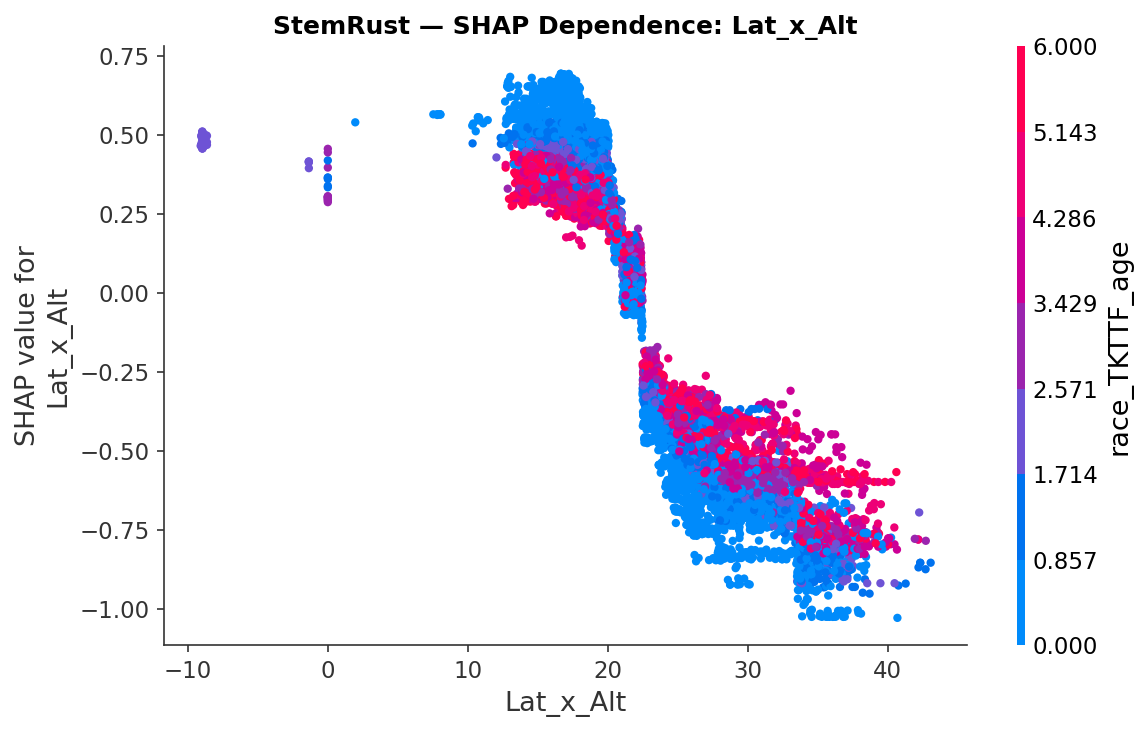
\includegraphics[width=\textwidth]{StemRust_shap_dep_1_Lat_x_Alt.png}
\caption{Stem: Lat$\times$Alt}
\end{subfigure}%
\begin{subfigure}[t]{0.33\textwidth}
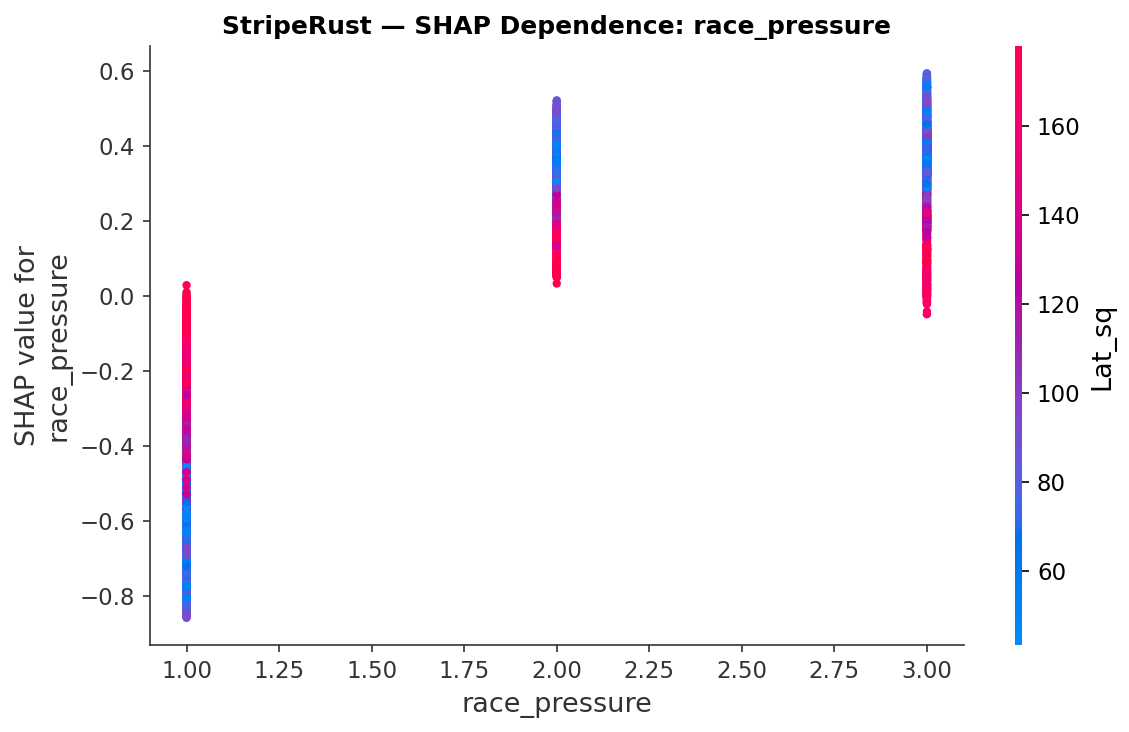
\includegraphics[width=\textwidth]{StripeRust_shap_dep_1_race_pressure.png}
\caption{Stripe: race\_pressure}
\end{subfigure}%
\begin{subfigure}[t]{0.33\textwidth}
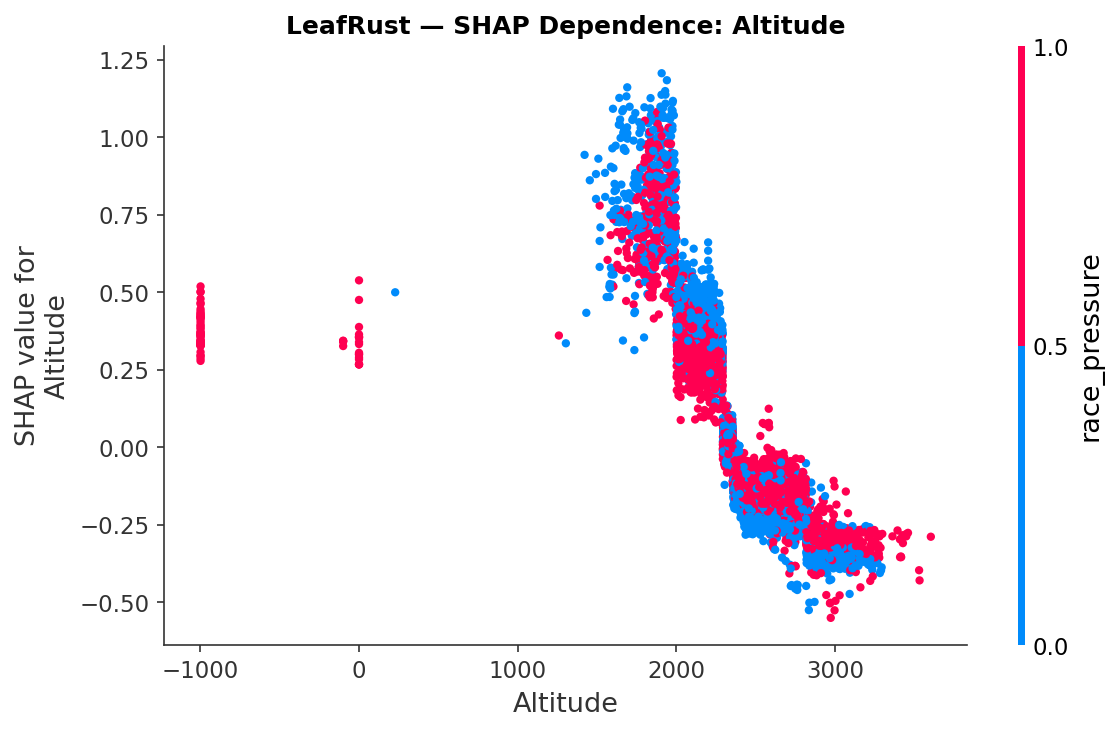
\includegraphics[width=\textwidth]{LeafRust_shap_dep_1_Altitude.png}
\caption{Leaf: Altitude}
\end{subfigure}
\caption{SHAP dependence plots for the top feature of each rust type. (a) Stem rust: Lat$\times$Alt shows a clear sigmoid transition---surveys with Lat$\times$Alt $<$ 15 (southern lowlands) receive positive SHAP (higher disease risk), with color indicating TKTTF race age as a secondary interaction. (b) Stripe rust: race\_pressure shows discrete levels (1--3) with strong positive SHAP at higher pressure levels, confirming that race regime is the primary driver. (c) Leaf rust: Altitude shows a pronounced non-linear decline from positive SHAP at ${\sim}$1800\,m to negative SHAP above ${\sim}$2500\,m, consistent with temperature-mediated prevalence patterns.}
\label{fig:shap_dep}
\end{figure*}

The stem rust dependence plot (\cref{fig:shap_dep}a) reveals a clear sigmoid transition: surveys with Lat$\times$Alt $<$ 15 (corresponding to southern, lower-altitude locations) receive strongly positive SHAP values (higher predicted disease risk), while those above ${\sim}$25 receive negative values. The color gradient (TKTTF race age) shows that the interaction with race dynamics modulates the spatial signal: in post-TKTTF years, the southern lowland risk is amplified.

The stripe rust plot (\cref{fig:shap_dep}b) shows that race\_pressure operates as an almost binary switch: level 1 (low pressure, inter-epidemic years) strongly suppresses predictions, while levels 2--3 (epidemic periods: PstS6 2010--11, PstS11 2016--18) strongly promote them. This explains why the baseline logistic model fails for stripe rust---it has no access to race information.

The leaf rust altitude dependence (\cref{fig:shap_dep}c) shows a pronounced non-linear relationship: positive SHAP at lower altitudes ($<$2000\,m asl), transitioning to negative SHAP at higher altitudes ($>$2500\,m asl). The color (race\_pressure) shows that this altitude gradient is modulated by temporal disease pressure, with post-2014 surveys showing slightly suppressed leaf rust at all altitudes, consistent with the secular decline.

\subsection{Features That Do Not Help}

Several feature categories contributed minimal predictive signal:

\noindent\textbf{Raw NDVI}: Ranked low for all rust types (SHAP $<$ 0.03). The NDVI anomaly and interaction features provided marginally more signal for stem rust but remained in the bottom half of feature rankings.

\noindent\textbf{ERA5 climate features}: Contributed meaningfully only for stem rust (+0.011 AUC). For stripe and leaf rust, climate variables added noise, and the best models exclude them entirely.

\noindent\textbf{Cyclical month encoding} (sin/cos): Near-zero SHAP values across all rust types, as the temporal signal is better captured by the more informative day-of-year and bi-weekly period features.

% ============================================================
\section{Discussion}
\label{sec:discussion}

\subsection{Why Feature Engineering Matters More Than Model Complexity}

The dominant source of improvement over the baseline comes from feature engineering, not model architecture. The four original features (latitude, longitude, altitude, days into season) capture only linear spatial and temporal trends. Our engineered features capture three critical dimensions the baseline misses:

\textit{Host--pathogen interactions}: The cultivar susceptibility and race regime features encode the boom-and-bust cycles that drive inter-annual variability---the primary reason the baseline fails for stripe and leaf rust.

\textit{Non-linear spatial structure}: The interaction terms (latitude$\times$altitude, etc.) capture the complex geographic patterns of disease risk that a linear model cannot represent, such as the altitude-dependent temperature regime varying with latitude.

\textit{Local epidemic context}: The spatial-temporal lag features provide direct information about ongoing disease spread in the neighborhood, converting each survey from an isolated point prediction into a spatially contextualized assessment.

The fact that TabNet (a deep learning model with implicit feature interaction learning) underperforms hand-crafted tree models by 6--8 AUC points underscores that domain knowledge, not model capacity, is the binding constraint at this data scale.

\subsection{Operational Implications}

The optimal decision thresholds (stem: 0.18, stripe: 0.35, leaf: 0.10) are all below the standard 0.5, reflecting the asymmetric costs of disease surveillance: missing a true outbreak (false negative) is far more costly than triggering unnecessary inspection (false positive). The dramatic F1 improvement for leaf rust (0.094 $\rightarrow$ 0.516) demonstrates that threshold calibration is essential for rare-disease prediction and should be standard practice in agricultural surveillance systems.

The spatial generalization results suggest that models trained on well-surveyed regions (Arsi, Bale, Shewa zones) can provide useful predictions for less-surveyed peripheral areas, supporting extension of the early warning system to undersampled regions.

\subsection{Limitations and Future Work}

\textbf{Temporal scope}: Our evaluation covers 2010--2019. Post-2019 pathogen race dynamics (e.g., new stem rust races emerging from 2019) may require model retraining.

\textbf{Feature availability}: Several of our most important features (cultivar identity, growth stage) require field-level observation and cannot be obtained remotely. This limits fully automated prediction but aligns with the existing RustTracker surveillance workflow.

\textbf{Spatial resolution}: ERA5 climate data at 0.25$^\circ$ (${\sim}$28\,km) resolution may miss local microclimatic variation relevant to disease in the topographically complex Ethiopian highlands. Higher-resolution climate products could improve the contribution of environmental features.

\textbf{Mechanistic integration}: Our purely data-driven approach could be complemented by mechanistic spore dispersal models~\cite{meyer2021} to incorporate atmospheric transport dynamics, potentially improving predictions during epidemic onset when lag features are not yet available.

% ============================================================
\section{Conclusion}
\label{sec:conclusion}

We demonstrate that machine learning models with domain-informed feature engineering substantially improve wheat rust disease prediction in Ethiopia compared to the logistic regression baseline of Meyer et al.\ (2021). Our best models achieve AUC-ROC improvements of +0.061 (stem rust), +0.121 (stripe rust), and +0.160 (leaf rust), with consistent gains across individual years and robust spatial generalization. SHAP analysis reveals epidemiologically interpretable prediction drivers: stem rust is driven by location--timing interactions, stripe rust by pathogen race dynamics, and leaf rust by altitude-mediated spatial structure. These findings provide actionable insights for the Ethiopian wheat rust early warning system, including race-informed surveillance prioritization, altitude-targeted variety deployment, and threshold-optimized decision support for all three rust types.

{\small
\bibliographystyle{ieeenat_fullname}
\begin{thebibliography}{9}

\bibitem{meyer2021}
M.~Meyer, N.~Bacha, T.~Tesfaye, Y.~Alemayehu, E.~Abera, B.~Hundie, G.~Woldeab, B.~Girma, A.~Gemechu, T.~Negash, T.~Mideksa, J.~Smith, M.~Jaleta, D.~Hodson, and C.~A.~Gilligan.
\newblock Wheat rust epidemics damage {E}thiopian wheat production: A decade of field disease surveillance reveals national-scale trends in past outbreaks.
\newblock {\em PLoS ONE}, 16(2):e0245697, 2021.

\bibitem{era5}
H.~Hersbach, B.~Bell, P.~Berrisford, S.~Hirahara, A.~Hor\'{a}nyi, J.~Mu\~{n}oz-Sabater, J.~Nicolas, C.~Peubey, R.~Radu, D.~Schepers, A.~Simmons, C.~Soci, S.~Abdalla, X.~Abellan, G.~Balsamo, P.~Bechtold, G.~Biavati, J.~Bidlot, M.~Bonavita, G.~De~Chiara, P.~Dahlgren, D.~Dee, M.~Diamantakis, R.~Dragani, J.~Flemming, R.~Forbes, M.~Fuentes, A.~Geer, L.~Haimberger, S.~Healy, R.~J.~Hogan, E.~Holm, M.~Janiskov\'{a}, S.~Keeley, P.~Laloyaux, P.~Lopez, C.~Lupu, G.~Radnoti, P.~de~Rosnay, I.~Rozum, F.~Vamborg, S.~Villaume, and J.-N.~Th\'{e}paut.
\newblock The {ERA5} global reanalysis.
\newblock {\em Quarterly Journal of the Royal Meteorological Society}, 146(730):1999--2049, 2020.

\bibitem{roelfs1992}
A.~P.~Roelfs, R.~P.~Singh, and E.~E.~Saari.
\newblock {\em Rust diseases of wheat: concepts and methods of disease management}.
\newblock CIMMYT, Mexico, D.F., 1992.

\bibitem{optuna}
T.~Akiba, S.~Sano, T.~Yanase, T.~Ohta, and M.~Koyama.
\newblock Optuna: A next-generation hyperparameter optimization framework.
\newblock In {\em Proceedings of the 25th ACM SIGKDD International Conference on Knowledge Discovery \& Data Mining}, pp.\ 2623--2631, 2019.

\bibitem{lundberg2020}
S.~M.~Lundberg, G.~Erion, H.~Chen, A.~DeGrave, J.~M.~Prutkin, B.~Nair, R.~Katz, J.~Himmelfarb, N.~Bansal, and S.-I.~Lee.
\newblock From local explanations to global understanding with explainable {AI} for trees.
\newblock {\em Nature Machine Intelligence}, 2(1):56--67, 2020.

\bibitem{tabnet}
S.~O.~Arik and T.~Pfister.
\newblock {TabNet}: Attentive interpretable tabular learning.
\newblock In {\em Proceedings of the AAAI Conference on Artificial Intelligence}, vol.\ 35, pp.\ 6679--6687, 2021.

\end{thebibliography}
}

\end{document}
